\RequirePackage[log]{snapshot}
\documentclass{greaseproof}
\usepackage{lipsum}

\usepackage{tikz}
\usetikzlibrary{calc}

\newcommand{\loremipsum}{ {\color{gray}  Lorem ipsum dolor sit amet, consectetur adipiscing elit. Suspendisse nisl purus, ultricies et ante quis, iaculis imperdiet justo. Proin tristique turpis a tortor eleifend lobortis. Vestibulum odio nisi, tempor sed scelerisque ac, aliquet a lorem. Proin ullamcorper nibh eget augue placerat lobortis. Quisque ac commodo libero, fringilla dictum purus. Proin nec massa vitae lorem eleifend lacinia. Praesent rhoncus ultricies ullamcorper. Fusce vel viverra purus, nec rhoncus massa. Etiam nisl lorem, cursus vel est sit amet, mattis venenatis magna. Vestibulum id risus sit amet nisi congue ultrices id nec ex. } }
\begin{document}

\input{blurbs/page-1-5}

% section 1
\section{Aksjomatyka}
Tekst podsekcji Aksjomatyka. \loremipsum
%

\subsection{Aksjomaty Euklidesa}
\subsection{Księga I}	
\subsubsection{Definicje}	
\begin{enumerate}	
    \item [1.1] Definicja ... % Definicja 1. % Punkt to jest to, co nie składa się z części.
    \item [1.2] Definicja ... % Definicja 2. % Linia jest długością bez szerokości.
    \item [1.3] Definicja ... % Definicja 3. % Końcami linii są punkty.
    \item [1.4] Definicja ... % Definicja 4. % Linia jest prosta, jeżeli położona jest między swoimi punktami w równym i jednostajnym kierunku.
    \item [1.5] Definicja ... % Definicja 5. % Powierzchnia jest to, co ma tylko długość i szerokość.
    \item [1.6] Definicja ... % Definicja 6. % Krawędzie powierzchni są liniami.
    \item [1.7] Definicja ... % Definicja 7. % Płaska powierzchnia albo płaszczyzna jest ta, na której biorąc gdziekolwiek dwa punkty linia prosta między tymi punktami cała leży na tej powierzchni.
    \item [1.8] Definicja ... % Definicja 8. % Kąt płaski to nachylenie dwóch linii na płaszczyźnie w miejscu, w którym jedna spotyka drugą i nie leżą w linii prostej.
    \item [1.9] Definicja ... % Definicja 9. % Kiedy linie są proste i tworzą kąt, wtedy kąt zwany jest prostoliniowym.
    \item [1.10] Definicja ... % Definicja 10. % Kiedy linia prosta padająca na drugą linie prostą, tworzy z nią kąty przyległe równe między sobą, to każdy z kątów równych nazywamy prostym, a padająca linia prostą nazywa się prostopadłą do tej linii, na którą pada.
    \item [1.11] Definicja ... % Definicja 11. % Kąt rozwarty jest większy od kąta prostego.
    \item [1.12] Definicja ... % Definicja 12. % Kąt ostry jest mniejszy od kąta prostego.
    \item [1.13] Definicja ... % Definicja 13. % Kresem albo granicą jest to, na czym się dana rzecz kończy.
    \item [1.14] Definicja ... % Definicja 14. % Figurą nazywamy to co jest ograniczone granicą lub granicami.
    \item [1.15] Definicja ... % Definicja 15. % Koło jest figurą płaską zawarta linią zwaną okręgiem, do której wszystkie linie proste poprowadzone z jednego punktu wewnątrz figury położonego, są między sobą równe.
    \item [1.16] Definicja ... % Definicja 16. % I ten punkt nazywa się centrum lub środkiem koła.
    \item [1.17] Definicja ... % Definicja 17. % Średnicą koła jest każda linia narysowana przez środek koła, przedłużona w dwóch kierunkach do jego obwodu, przepoławiająca go.
    \item [1.18] Definicja ... % Definicja 18. % Półokręgiem jest figura zawarta między średnicą i częscia okręgu odciętą tą średnicą. Środek półokregu jest też środkiem okręgu.
    \item [1.19] Definicja ... % Definicja 19. % Figury prostokreślne to figury ograniczone prostymi. Trójkąt to figura prostokreślna ograniczona trzema prostymi. Czworobok lub czworokąt to figura prostokreślna, która jest ograniczona czterema prostymi. Wielobok lub wielokąt to figura prostokreślna ograniczona więcej niż czterema prostymi.
    \item [1.20] Definicja ... % Definicja 20. % Trójkąt równoboczny to trójkąt, który ma trzy boki równe. Trójkąt równoramienny to trójkąt, który ma tylko dwa boki równe. Trójkąt różnoboczny to trójkąt, który ma trzy boki różne.
    \item [1.21] Definicja ... % Definicja 21. % Ponadto: trójkąt prostokątny to trójkąt, który na kąt prosty. Trójkąt rozwartokątny to trójkąt, który ma kąt rozwarty. Trójkąt ostrokątny to trójkąt, który ma trzy kąty ostre.
    \item [1.22] Definicja ... % Definicja 22. % Kwadrat jest to czworobok mający równe boki i równe kąty. Prostokąt jest to czworobok mający kąty proste, ale boki nierówne. Romb (kwadrat ukośny) jest to czworobok mający równe boki, ale nie mający kątów prostych. Równoległobok jest to czworobok mający boki przeciwległe równe, ale nie mający katów prostych. Wszystkie czworoboki inne niż wyżej wymienione nazywamy czworokątami.
    \item [1.23] Definicja ... % Definicja 23. % Linie równoległe, czyli mówiąc krócej równoległe są to proste, które leżą na tej samej płaszczyźnie i przedłużone z obu stron w nieskończoność, z żadnej strony nie przetną się.
\end{enumerate}	
	
\subsubsection{Postulaty}	
\begin{enumerate}	
    \item [1.1] Przez każde dwa punkty przechodzi prosta.
    \item [1.2] Postulat ... % Postulat 2. % Ograniczoną prostą można przedłużyć nieskończenie.
    \item [1.3] Postulat ... % Postulat 3. % Można zakreślić okrąg z któregokolwiek punktu jako środka dowolną odległością.
    \item [1.4] Wszystkie kąty proste są sobie równe.
    \item [1.5] Postulat ... % Postulat 5. % Jeżeli prosta przecinająca dwie proste tworzy z nimi kąty jednostronnie wewnętrzne o sumie mniejszej niż dwa kąty proste, to te dwie proste przedłużone nieskończenie przecinają się po tej stronie, po której znajdują się kąty o sumie mniejszej od dwóch kątów prostych.
\end{enumerate}	
	
Jak łatwo zauważyć, sformułowanie ostatniego postulatu używa więcej słów niż pozostałe razem wzięte; wbrew przekonaniu, że postulaty miały wyrażać treści oczywiste i proste.	
Piąty postulat wydawał się bardziej skomplikowany, więc nasuwał podejrzenie, że wynika z poprzednich czterech.	
Zauważył to już Proklos zwany Diadochem (410-485):
\index[persons]{Proklos zwany Diadochem}%
\emph{,,Nie jest możliwe, aby uczony tej miary co Euklides godził się na obecność tak długiego postulatu w aksjomatyce -- obecność postulatu wzięła się z pospiesznego kończenia przez niego Elementów, tak aby zdążyć przed nadejściem słusznie oczekiwanej rychłej śmierci; my zatem -- czcząc jego pamięć -- powinniśmy ten postulat usunąć lub co najmniej znacznie uprościć.''}	
	
Wiele osób próbowało stawić czoło wyzwaniu postawionemu przez Proklosa.	
Bezskutecznie, ponieważ piąty postulat jest niezależny od pozostałych, zaś zastąpienie go jego zaprzeczeniem prowadzi do geometrii nieeuklidesowych.	
Piszą o tym Audin \cite[s. 13]{audin_2003}.
	
\subsubsection{Pojęcia pierwotne}	
\begin{enumerate}	
    \item [1.1] Wyrażenia, które są równe się temu samemu wyrażeniowi, są sobie równe.
    \item [1.2] Równania można dodawać stronami.
    \item [1.3] Równania można odejmować stronami.
    \item [1.4] Wyrażenia, które się pokrywają, są sobie równe.
    \item [1.5] Całość jest większa od części.
\end{enumerate}	
	
\subsubsection{Twierdzenia}	
\begin{enumerate}	
    \item [1.1] Skonstruować trójkąt równoboczny o zadanym boku.
    \item [1.2] Twierdzenie ... % Twierdzenie 2. % Skonstruuj odcinek równy danemu odcinkowi którego koniec jest zadanym punktem.
    \item [1.3] Skonstruować różnicę dwóch odcinków.
    \item [1.4] Twierdzenie ... \hfill \emph{(przystawanie bok-kąt-bok)} % Twierdzenie 4. % Jeśli dwa trójkąty mają dwa boki odpowiednio równe dwóm innym, i jeżeli kąty zawarte między bokami równoległymi są równe, wtedy ich podstawy również są sobie równe i pozostałe kąty równe są odpowiednim kątom.
    \index{cecha przystawania!bok-kąt-bok}%
    \item [1.5] Twierdzenie ... % Twierdzenie 5. % W trójkątach równoramiennych kąty przy podstawie są sobie równe oraz kąty powstałe przez przedłużenie boków równych są sobie równe.
    \item [1.6] Boki trójkąta leżące naprzeciw przystających kątów są przystające.
    \item [1.7] Twierdzenie ... % Twierdzenie 7. % Na tej samej podstawie i z tej samej strony nie mogą być wykreślone dwa trójkąty takie, żeby boki w tych trójkątach przy obydwu końcach wspólnej podstawy były między sobą równe.
    \item [1.8] Twierdzenie ... \hfill \emph{(przystawanie bok-bok-bok)} % Twierdzenie 8. % Jeżeli dwa boki jednego trójkąta są równe dwóm bokom drugiego trójkąta, to kąty zawarte między równymi bokami są sobie równe.
    \index{cecha przystawania!bok-bok-bok}%
    \item [1.9] Podzielić dany kąt na dwie równe części.
    \item [1.10] Podzielić dany odcinek na dwie równe części.
    \item [1.11] Twierdzenie ... % Twierdzenie 11. % Z punktu danego na danej linii prostej wyprowadzić linie prostopadłą do danej linii prostej.
    \item [1.12] Twierdzenie ... % Twierdzenie 12. % Z punktu danego leżącego poza linią prostą nieograniczoną, wyprowadzić prostą linię prostopadłą do niej.
    \item [1.13] Twierdzenie ... % Twierdzenie 13. % Jeżeli linia prosta przecinająca drugą prostą tworzy z nią dwa kąty, to są one proste, albo równe dwóm kątom prostym.
    \item [1.14] Twierdzenie ... % Twierdzenie 14. % Jeżeli przy linii prostej i przy punkcie na niej leżącym dwie linie proste nie po jednej stronie położone czynią kąty przyległe równe dwóm kątom prostym, to te linie proste będą w tym samym kierunku.
    \item [1.15] Twierdzenie ... % Twierdzenie 15. % Jeżeli dwie linie proste przecinają się, to utworzone przez nie kąty przeciwległe są sobie równe.
    \item [1.16] Twierdzenie ... % Twierdzenie 16. % W dowolnym trójkącie kąt zewnętrzny powstały przez przedłużenie jednego boku jest większy od każdego z dwóch kątów wewnętrznych przeciwległych jemu.
    \item [1.17] W każdym trójkącie suma dwóch kątów jest mniejsza od $\pi$.
    \item [1.18] Twierdzenie ... % Twierdzenie 18. % W każdym trójkącie bok większy przeciwległy jest kątowi większemu.
    \item [1.19] Twierdzenie ... % Twierdzenie 19. % W każdym trójkącie kąt większy przeciwległy jest bokowi większemu.
    \item [1.20] Twierdzenie ... % Twierdzenie 20. % W każdym trójkącie suma dwóch dowolnych boków jest większa od boku trzeciego.
    \item [1.21] Twierdzenie ... % Twierdzenie 21. % Jeżeli z końców jednego boku trójkąta poprowadzone będą dwie linie proste wewnątrz trójkąta, aż do zejścia się z sobą, to te dwie linie proste będą mniejsze od dwóch pozostałych boków trójkąta, lecz zawierać jednak będą kąt większy od kąta zawartego między pozostałymi bokami trójkąta.
    \item [1.22] Twierdzenie ... % Twierdzenie 22. % Aby z trzech danych linii prostych wykreślić trójkąt, potrzeba aby z tych trzech danych linii prostych suma dwóch którychkolwiek była większa od trzeciej.
    \item [1.23] Twierdzenie ... % Twierdzenie 23. % Na danej linii prostej i punkcie na niej danym wykreślić kąt prostokreślny równy kątowi prostokreślnemu danemu.
    \item [1.24] Twierdzenie ... % Twierdzenie 24. % Jeżeli dwa boki jednego trójkąta, są równe dwóm bokom trójkąta drugiego, z kątów zaś między bokami równymi jeden większy jest od drugiego; to będzie też podstawa jednego trójkąta większa od podstawy drugiego trójkąta.
    % TODO: https://en.wikipedia.org/wiki/Hinge_theorem
    \item [1.25] Twierdzenie ... % Twierdzenie 25. % Jeżeli dwa boki jednego trójkąta, są równe dwóm bokom trójkąta drugiego, lecz podstawa jednego trójkąta większa jest od podstawy drugiego trójkąta, to i kąty między bokami równymi zawarte będą jeden większy od drugiego.
    \item [1.26] Twierdzenie ... % Twierdzenie 26. % Jeżeli dwa kąty jednego trójkąta są równe dwóm kątom drugiego trójkąta, i bok jeden przyległy obydwu kątom, albo jednemu w pierwszym trójkącie równa się bokowi jednemu przyległemu obydwu katom, albo jednemu w drugim trójkącie; będą i dwa boki pozostałe równe dwóm bokom pozostałym i kąt trzeci w jednym trójkącie będzie równy katowi trzeciemu w drugim trójkącie.
    \item [1.27] Twierdzenie ... % Twierdzenie 27. % Jeżeli na dwie linie proste, pada linia prosta czyniąca kąty naprzemian równe między sobą, to te dwie linie proste będą równoległe.
    \item [1.28] Twierdzenie ... % Twierdzenie 28. % Jeśli linia prosta opada na dwie linie proste, tworząc kąt zewnętrzny równy wewnętrznemu i przeciwny do kąta na tym samym boku lub suma kątów wewnętrznych na tym samym boku jest równa dwóm kątom prostym, wtedy linie proste są równoległe do siebie.
    \item [1.29] Twierdzenie ... % Twierdzenie 29. % Linia prosta opada na równoległą linie prostą tworząc alternatywne kąty równe sobie, kąt zewnętrzny równy wewnętrznemu i przeciwległy i suma kątów wewnętrznych na tym samym boku jest równa dwóm kątom prostym.
    \item [1.30] Twierdzenie ... % Twierdzenie 30. % Linie proste, które są równoległe do linii prostej są również równoległe do siebie.
    \item [1.31] Twierdzenie ... % Twierdzenie 31. % Poprowadzić przez dany punkt linię prostą równoległą względem danej lini prostej.
    \item [1.32] Twierdzenie ... % Twierdzenie 32. % W jakimkolwiek trójkącie, jeśli jeden z boków jest znany wtedy kąt zewnętrzny jest równy sumie dwóch kątów wewnętrznych i przeciwnych i suma trzech wewnętrznych kątów trójkąta jest równa dwóm kątom prostym.
    \item [1.33] Twierdzenie ... % Twierdzenie 33. % Linie proste, które łączą końce równych i równoległych linii prostych w tym samym kierunku są sobie równe i równoległe.
    \item [1.34] Twierdzenie ... % Twierdzenie 34. % W równoległobokach boki i kąty przeciwne są między sobą równe, a przekątna dzieli je na dwie równe części.
    \item [1.35] Twierdzenie ... % Twierdzenie 35. % Równoległoboki, które są na takiej samej podstawie i są porównywalne są sobie równe.
    \item [1.36] Twierdzenie ... % Twierdzenie 36. % Równoległoboki, które mają równe podstawy i są porównywalne są sobie równe.
    \item [1.37] Twierdzenie ... % Twierdzenie 37. % Trójkąty, które mają takie same podstawy i są porównywalne są sobie równe.
    \item [1.38] Twierdzenie ... % Twierdzenie 38. % Trójkąty, których podstawy są równe i są one porównywalne są sobie równe.
    \item [1.39] Twierdzenie ... % Twierdzenie 39. % Równe trójkąty, które są na takich samych podstawach i mające te same boki również są porównywalne.
    \item [1.40] Twierdzenie ... % Twierdzenie 40. % Równe trójkąty, które mają takie same podstawy i mają te same boki również są porównywalne.
    \item [1.41] Twierdzenie ... % Twierdzenie 41. % Jeśli równoległobok i trójkąt mają tą samą podstawę i są tymi samymi liniami zakończone, to trójkąt jest połową równoległoboku.
    \item [1.42] Twierdzenie ... % Twierdzenie 42. % Skonstruować równoległobok równy danemu trójkątowi o podanym prostoliniowym kącie.
    \item [1.43] Twierdzenie ... % Twierdzenie 43. % W każdym równoległoboku, dopełnienia równoległoboków koło przekątnych położonych są między sobą równe.
    \item [1.44] Twierdzenie ... % Twierdzenie 44. % Na danej linii prostej wykreślić równy danemu równoległobok, którego jeden kąt będzie równy danemu.
    \item [1.45] Twierdzenie ... % Twierdzenie 45. % Wykreślić równy danej figurze prostokreślny równoległobok, którego jeden kąt będzie równy danemu.
    \item [1.46] Skonstruować kwadrat.
    \item [1.47] Twierdzenie ... \hfill \emph{(twierdzenie Pitagorasa)} % Twierdzenie 47. % W trójkącie prostokątnym, kwadrat zbudowany na boku przeciwnym kątowi prostemu, równy jest kwadratom zbudowanym na bokach, które kąt prosty zawierają.
    \index{twierdzenie!Pitagorasa}
    \item [1.48] Twierdzenie ... \hfill \emph{(twierdzenie odwrotne do twierdzenia Pitagorasa)} % Twierdzenie 48. % Jeżeli kwadrat zbudowany na jednym z boków trójkąta, jest równy kwadratom wykreślonym na dwóch pozostałych bokach trójkąta, to kąt zawarty między dwoma pozostałymi bokami będzie prosty.
\end{enumerate}

%
\input{axioms/axioms-euclid-2}
%

\subsection{Księga III}
\subsubsection{Definicje}
\begin{enumerate}
    \item [3.1] Dwa okręgi są przystające, kiedy mają równe średnice (lub równoważnie, promienie).
    \item [3.2] Definicja ...
    % Definicja 2. % Mówi się, że linia prosta dotyka koła, gdy będąc styczną z kołem przedłużona z obydwu stron nie przecina się z żadnej strony okręgu koła.
    \item [3.3] Dwa okręgi nazywamy stycznymi, kiedy mają dokładnie jeden punkt wspólny.
    \item [3.4] Definicja ...
    % Definicja 4. % Mówi się, że linie proste równoodległe są od środka koła, gdy prostopadłe ze środka koła na nie spuszczone są równe.
    \item [3.5] Definicja ...
    % Definicja 5. % Mówi się, że ta linia prosta bardziej jest odległa od środka koła, na którą prostopadła ze środka koła spuszczona jest większa.
    \item [3.6] Definicja ...
    % Definicja 6. % Odcinkiem koła jest figura czyli część koła ograniczona linią prostą i okręgiem koła.
    \item [3.7] Definicja ...
    % Definicja 7. % Kąt zaś odcinka jest ten, który się linią prostą i okręgiem koła zawiera.
    \item [3.8] Definicja ...
    % Definicja 8. % Jeżeli na okręgu koła wzięty będzie punkt i od niego będą poprowadzone linie proste do końców linii prostej za podstawę odcinkami służącej, kąt między tymi liniami prostymi zawarty jest kątem w odcinku.
    \item [3.9] Definicja ...
    % Definicja 9. % Kiedy zaś linie proste kąt zawierające zajmują część okręgu, mówi się, że kąt ten opiera się na okręgu koła.
    \item [3.10] Definicja ...
    % Definicja 10. % Jeżeli kąt ma swój wierzchołek we środku koła; figura czyli część koła zawarta między ramionami tegoż koła, to jest między promieniami i łukiem koła nazywa się wycinkiem koła.
    \item [3.11] Definicja ...
    % Definicja 11. % Odcinkami podobnymi kół nazywają się te, które zajmują kąty równe, lub w których kąty są równe między sobą.
\end{enumerate}

\subsubsection{Twierdzenia}
\begin{enumerate}
    \item [3.1] Skonstruować środek danego okręgu. 
    \item [3.2] Twierdzenie ...
    % Twierdzenie 2. % Jeżeli na okręgu obierzemy dwa gdziekolwiek punkty, linia prosta łącząca te punkty padnie wewnątrz koła.
    \item [3.3] Twierdzenie ...
    % Twierdzenie 3. % Jeżeli w kole linia prosta przez środek poprowadzona przecina linie nie przez środek poprowadzoną na dwie równe części, będzie pierwsza prostopadła do drugiej; i jeżeli pierwsza jest prostopadła do drugiej, przecina ja na dwie równe części.
    \item [3.4] Twierdzenie ...
    % Twierdzenie 4. % Jeżeli w kole dwie linie proste, nie przez środek koła poprowadzone przecinają się nawzajem, nie przetną się na dwie równe części.
    \item [3.5] Dwa okręgi, które się przecinają, nie mogą być współśrodkowe. 
    \item [3.6] Twierdzenie ...
    % Twierdzenie 6. % Jeżeli dwa koła dotykają się wzajemnie, to wspólnego środka mieć nie mogą.
    \item [3.7] Twierdzenie ...
    % Twierdzenie 7. % Jeżeli na średnicy koła wzięty będzie punkt którykolwiek oprócz średnicy koła i od tego punktu poprowadzone linie proste do okręgu, ze wszystkich linii największa będzie część średnicy, na której znajduje się środek koła, a najmniejsza pozostała część średnicy, z innych zaś linii prostych każda bliższa przechodząca przez środek koła, większa będzie od odleglejszej, z tego na koniec punktu dwie tylko równe linie proste z obydwu stron najmniejszej linii prostej mogą być do okręgu poprowadzone.
    \item [3.8] Twierdzenie ...
    % Twierdzenie 8. % Jeżeli z punktu zewnątrz koła obranego, poprowadzone będą do okręgu linie proste, z których jedna przechodziła by przez środek koła a inne padały gdziekolwiek, z linii prostych padających na część okręgu wklęsłą, największa jest linia poprowadzona przez środek koła, z innych zaś linii każda bliższa przechodzącej przez środek jest większa od odleglejszej. Lecz z linii padających na cześć okręgu wypukłą, najmniejsza jest linia prosta zawarta między punktem zewnętrz koła i średnicą, z innych zaś linii prostych każda bliższa najmniejszej, mniejsza jest odleglejsza; na koniec dwie tylko równe linie proste z tego punktu po obydwu stronach najmniejszej linii prostej mogą być do okręgu poprowadzone.
    \item [3.9] Twierdzenie ...
    % Twierdzenie 9. % Jeżeli z punktu danego wewnątrz koła poprowadzimy do okręgu więcej niż dwie linie proste i te proste są miedzy sobą równe, punkt ten będzie środkiem koła.
    \item [3.10] Dwa okręgi, które się przecinają, przecinają się w dwóch punktach. 
    \item [3.11] Twierdzenie ...
    % Twierdzenie 11. % Jeżeli dwa koła stykają się ze sobą wewnątrz, linia łącząca środki tychże kół przedłużona pada na punkt dotykania się kół.
    \item [3.12] Twierdzenie ...
    % Twierdzenie 12. % Jeżeli dwa koła dotykają się ze sobą zewnętrznie, to linia prosta łącząca ich środki przechodzi przez punkt dotykania się.
    \item [3.13] Twierdzenie ...
    % Twierdzenie 13. % Okrąg koła nie może dotykać okręgu drugiego koła w więcej niż jednym punkcie, nieważne jest czy dotkniecie jest zewnętrzne bądź wewnętrzne.
    \item [3.14] Twierdzenie ...
    % Twierdzenie 14. % W kole linie proste równe, na okręgu jego zakończone, są równoodległe od środka; i linie proste które na okręgu jego zakończone są równoodległe od środka, są też miedzy sobą równe.
    \item [3.15] Twierdzenie ...
    % Twierdzenie 15. % Ze wszystkich linii prostych w kole poprowadzonych i na okręgu jego zakończonych, największa jest średnica, z innych zaś każda bliższa środka koła, większa jest od odleglejszej; i z dwóch linii prostych nierównych, większa bliższa jest środka koła od mniejszej.
    \item [3.16] Twierdzenie ... 
    % Twierdzenie 16. % Prostopadła do średnicy koła z końca jej wyprowadzona, pada cała zewnątrz koła, a między tą prostopadłą i okręgiem żadna inna linia prosta nie pada; albo tak samo: okrąg koła przechodzi miedzy prostopadłą do średnicy i linią prostą, która ze średnicą kąt ostry jakokolwiek wielki zawiera, czyli która zawiera kąt jakokolwiek mały z prostopadłą do średnicy.
    \item [3.17] Skonstruować styczną do danego okręgu, która przechodzi przez dany punkt.
    \item [3.18] Twierdzenie ...
    % Twierdzenie 18. % Jeżeli linia prosta dotyka się okręgu koła, a ze środka koła wyprowadzona będzie linia prosta do punktu dotykania się, to ta będzie prostopadła do stycznej.
    \item [3.19] Twierdzenie ...
    % Twierdzenie 19. % Jeżeli linia prosta dotyka okręgu koła, z punktu zaś dotknięcia wyprowadzona będzie do tej stycznej prostopadła, to na prostopadłej będzie środek koła.
    \item [3.20] Twierdzenie ...
    % Twierdzenie 20. % W kole, kąt mający wierzchołek we środku jest podwojeniem kata mającego swój wierzchołek na okręgu koła, gdyż tę samą podstawę okręgu mają za podstawę, czyli to samo gdy ramionami swymi tej samej części okręgu obejmują.
    \item [3.21] Twierdzenie ...
    % Twierdzenie 21. % Kąty w tym samym odcinku koła są między sobą równe.
    \item [3.22] Twierdzenie ...
    % Twierdzenie 22. % Kąty przeciwne czworokąta w koło wpisane są równe dwóm kątom prostym.
    \item [3.23] Twierdzenie ...
    % Twierdzenie 23. % Na tej samej linii prostej nie można wykreślić dwóch odcinków kół po tej samej stronie podobnych, które by nie przystawały do siebie.
    \item [3.24] Twierdzenie ...
    % Twierdzenie 24. % Wykreślone na równych liniach prostych podobne odcinki kół, są między sobą równe.
    \item [3.25] Twierdzenie ...
    % Twierdzenie 25. % Mając dany odcinek koła, opisać koła którego jest odcinkiem.
    \item [3.26] Twierdzenie ...
    % Twierdzenie 26. % W kołach równych, kąty równe w środkach lub przy okręgach wspierają się na równych łukach.
    \item [3.27] Twierdzenie ...
    % Twierdzenie 27. % W kołach równych, kąty we środkach lub przy okręgach, na równych łukach wspierające się, są między sobą równe.
    \item [3.28] Twierdzenie ...
    % Twierdzenie 28. % W kołach równych, cięciwy równe obejmują łuki równe, tak, że łuk większy większemu, mniejszy mniejszemu jest równy.
    \item [3.29] Twierdzenie ...
    % Twierdzenie 29. % W kołach równych, równe łuki obejmują cięciwy równe.
    \item [3.30] Podzielić dany Twierdzenie ...
    % Twierdzenie 30. % Dany łuk podzielić na dwie części.
    \item [3.31] Twierdzenie ...
    % Twierdzenie 31. % W kole, kąt w półkolu jest prosty; z katów zaś w odcinkach nierównych, kąt w większym odcinku mniejszy jest od prostego; a w mniejszym odcinku większy od prostego.
    \item [3.32] Twierdzenie ...
    % Twierdzenie 32. % Jeżeli okręgu koła dotyka linia prosta, z punktu zaś dotknięcia poprowadzona będzie cięciwa, kąty zawarte miedzy cięciwową i styczną, będą równe kątom w odcinkach koła na przemian.
    \item [3.33] Twierdzenie ...
    % Twierdzenie 33. % Na danej linii prostej wykreślić odcinek koła który by zawierał kąt równy kątowi danemu.
    \item [3.34] Twierdzenie ...
    % Twierdzenie 34. % Z koła danego oddzielić odcinek któryby zawierał kąt równy danemu kątowi.
    \item [3.35] Twierdzenie ...
    % Twierdzenie 35. % Jeżeli w kole dwie cięciwy przecinają się nawzajem, prostokąt zawarty odcinkami jednej cięciwy będzie równy prostokątowi zawartemu odcinkami drugiej cięciwy.
    \item [3.36] Twierdzenie ...
    % Twierdzenie 36. % Jeżeli z punktu za kołem obranego, poprowadzimy dwie linie proste, których jedna przecinałaby koło, a druga byłaby styczną; to prostokąt zawarty całą linia przecinającą i odcinkiem jej za kołem będzie równy kwadratowi ze stycznej.
    \item [3.37] Twierdzenie ...
    % Twierdzenie 37. % Jeżeli z dwóch linii prostych, od jednego punktu zewnątrz koła obranego poprowadzonych, jedna przecina koło, a druga pada na okrąg tego koła: i jeżeli prostokąt z całej linii przecinającej i odcinka jej za kołem będącego jest równy kwadratowi z linii padającej na okrąg koła, to linia będzie padająca na okrąg koła styczną.
\end{enumerate}

%
%

\subsubsection{Księga IV}
\paragraph{Definicje}
\begin{enumerate}
	\item [4.1] Definicja ...
	% Definicja 1. % Mówi się że figura prostokreślna wpisuje się w figurę prostokreślną, wtedy kiedy każdy kąt figury wpisanej dotyka się każdego boku figury, w który się wpisuje.
	\item [4.2] Definicja ...
	% Definicja 2. % Podobnie się mówi, że figura opisuje się na figurze, kiedy każdy bok figury opisanej dotyka każdego kąta figury na której się opisuje.
	\item [4.3] Definicja ...
	% Definicja 3. % Figura prostokreślna wpisuje się w koło, kiedy każdy kąt figury wpisanej dotyka okręgu koła.
	\item [4.4] Definicja ...
	% Definicja 4. % Figura prostokreślna opisuje się na kole kiedy każdy bok figury opisanej dotyka okręgu koła.
	\item [4.5] Definicja ...
	% Definicja 5. % Podobnież koło wpisuje się w figurę prostokreślną, kiedy każdy bok figury w którą koło się wpisuje, dotyka okręgu koła.
	\item [4.6] Definicja ...
	% Definicja 6. % Koło opisuje się na figurze prostokreślne wtedy gdy okrąg dotyka do każdego kąta figury na której opisujemy koło.
	\item [4.7] Definicja ...
	% Definicja 7. % Mówi się, że linie proste kreśli się w kole, gdy jej końce są na okręgu danego koła.
\end{enumerate}

\paragraph{Twierdzenia}
\begin{enumerate}
	\item [4.1] Wpisać odcinek krótszy od średnicy w dany okrąg.
	\item [4.2] Twierdzenie ...
	% Twierdzenie 2. % W dane koło wpisać trójkąt równoramienny względem danego trójkąt.
	\item [4.3] Twierdzenie ...
	% Twierdzenie 3. % Na danym kole opisać trójkąt równokątny względem danego trójkąta.
	\item [4.4] Twierdzenie ...
	% Twierdzenie 4. % W dany trójkąt wpisać koło.
	\item [4.5] Twierdzenie ...
	% Twierdzenie 5. % Na danym trójkącie opisać koło.
	\item [4.6] Wpisać kwadrat w dany okrąg.
	\item [4.7] Opisać kwadrat na danym okręgu.
	\item [4.8] Wpisać okrąg w dany kwadrat.
	\item [4.9] Opisać okrąg na danym kwadracie.
	\item [4.10] Wykreślić trójkąt równoramienny, którego kąt przy podstawie jest podwojeniem kąta przy wierzchołku (o kątach $\pi/5$, $2\pi/5$, $2\pi/5$).
	\item [4.11] Twierdzenie ...
	% Twierdzenie 11. % W dane koło wpisać pięciokąt równoboczny i równokątny.
	\item [4.12] Opisać pięciokąt równoboczny i równokątny na danym okręgu.
	\item [4.13] Wpisać okrąg w dany pięciokąt równoboczny i równokątny.
	\item [4.14] Opisać okrąg na danym pięciokącie równobocznym i równokątnym
	\item [4.15] Wpisać sześciokąt równoboczny i równokątny w dany okrąg.
	\item [4.16] Wpisać piętnastokąt równoboczny i równokątny w dany okrąg.
\end{enumerate}

%

% TODO: https://kpbc.umk.pl/dlibra/publication/37/edition/66/content
% TODO: Pojęcia pierwotne i aksjomaty Euklidesa nie są jednak idealne.
% TODO: Dlatego zamiast nich będziemy używać aksjomatów Hilberta podanych około 1899 roku.

% https://www.claymath.org/library/historical/euclid/
% BOOK I	Triangles, parallels, and area
% BOOK II	Geometric algebra
% BOOK III	Circles
% BOOK IV	Constructions for inscribed and circumscribed figures
% BOOK V	Theory of proportions
% BOOK VI	Similar figures and proportions
% BOOK VII	Fundamentals of number theory
% BOOK VIII	Continued proportions in number theory
% BOOK IX	Number theory
% BOOK X	Classification of incommensurables
% BOOK XI	Solid geometry
% BOOK XII	Measurement of figures
% BOOK XIII	Regular solids

%
%

\subsection{Aksjomaty Hilberta}
W aksjomatyce Hilberta (płaskiej geometrii euklidesowej) pojęciami pierwotnymi są punkt, prosta, płaszczyzna, relacja incydencji (leżeć na, zawierać się w), relacja uporządkowania (leżenia między) oraz relacja przystawania.

%

\subsubsection{Aksjomaty incydencji}
\begin{axiom}[incydencji, I1]
    Dla każdej pary punktów $A$ oraz $B$ istnieje dokładnie jedna prosta $l$, która przechodzi przez te punkty.
\end{axiom}

\begin{axiom}[incydencji, I2]
    Na każdej prostej istnieją co najmniej dwa punkty.
\end{axiom}

\begin{axiom}[incydencji, I3]
    Istnieją co najmniej trzy punkty, które nie są współliniowe.
\end{axiom}

,,Być współliniowym'' to synonim leżenia na jednej prostej.

\begin{proposition}
    Dwie różne proste mogą mieć co najwyżej jeden punkt wspólny.
\end{proposition}

\begin{definition}
    Dwie różne proste, które nie mają punktów wspólnych, nazywamy równoległymi.
    Każda prosta jest też równoległa do siebie.
\end{definition}

\begin{axiom}[Playfaira, P]
    Dla każdej prostej $l$ oraz punktu $A$, istnieje co najwyżej jedna prosta przechodząca przez $A$, równoległa do $l$.
\end{axiom}

John Playfair opublikował ten aksjomat w 1795 roku, chociaż już wtedy twierdził, że inni używali go przed nim (np. William Ludlam).
\index[persons]{Playfair, John}%
Aksjomat Playfaira jest równoważny z (piątym) postulatem Euklidesa i dlatego wiele osób próbowało wyprowadzić go z czterech wcześniejszych postulatów.
Za każdym razem okazywało się, że w ,,dowodzie'' użyte jest zdanie będące równoważnikiem piątego postulatu, na przykład:
\begin{itemize}
    \item suma kątów wewnętrznych każdego trójkąta jest kątem półpełnym,
    \item suma kątów wewnętrznych każdego trójkąta jest taka sama,
    \item istnieje trójkąt, którego suma kątów wewnętrznych jest kątem półpełnym,
    \item istnieją dwa trójkąty, które są do siebie podobne, ale nie przystające,
    \item na każdym trójkącie można opisać okrąg,
    \item jeśli trzy kąty wewnętrzne czworokąta są proste, to czwarty kąt także jest prosty,
    \item istnieje para prostych, które są w stałej odległości od siebie,
    \item dwie proste, które są równoległe do danej prostej, są też równoległe do siebie,
    \item twierdzenie Pitagorasa lub jego uogólnienie, twierdzenie cosinusów
    \item aksjomat Wallisa: nie ma górnego ograniczenia na pole trójkąta,
    \item kąty przy górnej podstawie czworokąta Saccheriego (czworokąta $ABCD$ o dwóch kątach prostych przy dolnej podstawie $AB$, w którym boki $AD$ i $BC$ mają równe długości) są proste,
    \item aksjomat Proklosa: jeśli prosta przecina jedną z dwóch równoległych prostych, to przecina także tę drugą.
\end{itemize}

\begin{example}
    Rozważmy geometrię, gdzie płaszczyzna składa się z pięciu punktów $A$, $B$, $C$, $D$, $E$ i leży na niej dziesięć różnych prostych, każda z nich przechodząca przez dokładnie dwa różne punkty.
    Wtedy proste $AB$ i $AC$ mają punkt wspólny $A$, chociaż obydwie są równoległe do prostej $DE$.
    Aksjomat Playfaira nie jest spełniony.
\end{example}

\begin{proposition}
    Aksjomaty incydencji I1, I2, I3 oraz aksjomat P (Playfaira) są od siebie niezależne.
\end{proposition}

Hartshorne \cite[s. 69-70]{hartshorne2000} konstruuje modele geometrii, w których spełnione są dowolne trzy, ale nie czwarty z nich.

\begin{proposition}
    Płaszczyzna rzutowa to taki zbiór punktów oraz prostych (podzbiorów zbioru punktów), że:
    \begin{itemize}
        \item przez dwa różne punkty przechodzi dokładnie jedna prosta,
        \item każde dwie proste mają punkt wspólny,
        \item każda prosta ma co najmniej trzy punkty i
        \item nie wszystkie punkty są współliniowe.
    \end{itemize}
    (Każdy z wymienionych aksjomatów jest niezależny od pozostałych, ze wszystkich razem wynikają aksjomaty incydencji).
    Każda płaszczyzna rzutowa ma co najmniej 7 punktów, dokładnie jedna płaszczyzna rzutowa ma dokładnie 7 punktów.
    Jeśli istnieje prosta, która ma $n+1$ punktów, to płaszczyzna ma $n^2 + n + 1$ punktów.
\end{proposition} % Hartshorne 71

\begin{example}[płaszczyzna Fana]
    Zbiór złożony z siedmiu elementów (,,punktów''), w którym wyróżniono rodzinę siedmiu podzbiorów (,,prostych'') spełniający następujące warunki:
    \begin{itemize}
        \item każde dwie różne proste mają dokładnie jeden punkt wspólny,
        \item każde dwa różne punkty należą do dokładnie jednej prostej
    \end{itemize}
    nazywamy płaszczyzną Fana.
    Jest przykładem płaszczyzny rzutowej, która nie spełnia aksjomatu Fana (że trzy punkty przekątne czworoboku zupełnego nie są współliniowe).
    \begin{figure}[H]
        \centering
        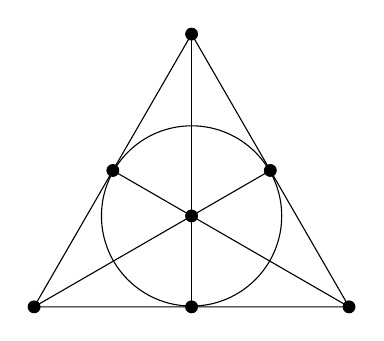
\begin{tikzpicture}[
        mydot/.style={
        draw,
        circle,
        fill=black,
        inner sep=1.5pt}
        ]
        \draw
        (0,0) coordinate (A) --
        (4cm,0) coordinate (B) --
        ($ (A)!.5!(B) ! {sin(60)*2} ! 90:(B) $) coordinate (C) -- cycle;
        \coordinate (O) at
        (barycentric cs:A=1,B=1,C=1);
        \draw (O) circle [radius=4cm*1.717/6];
        \draw (C) -- ($ (A)!.5!(B) $) coordinate (LC); 
        \draw (A) -- ($ (B)!.5!(C) $) coordinate (LA); 
        \draw (B) -- ($ (C)!.5!(A) $) coordinate (LB); 
        \foreach \Nodo in {A,B,C,O,LC,LA,LB}
        \node[mydot] at (\Nodo) {};    
    \end{tikzpicture}%
    \caption{Płaszczyzna Fana}
\end{figure}
\end{example}

W momencie pisania tego tekstu nie jesteśmy jeszcze zainteresowani geometrią rzutową, więc przytoczymy tylko wymagania wobec studenta, który ukończył kurs ,,Geometria III'' na uniwersytecie w Warszawie.

Zna pojęcie płaszczyzny rzutowej rzeczywistej (równoważne sformułowania), dwustosunku, definicję przekształceń rzutowych łańcuchów, stożkowych, pęków stycznych do stożkowych.
\index{dwustosunek}%
\index{pęk}%
\index{stożkowa}%
Zna i~potrafi stosować twierdzenia Steinera i Braikenridge'a-Maclaurina.
\index{twierdzenie!Steinera}%
\index{twierdzenie!Braikendridge'a-Maclaurina}%
Wie w jaki sposób określa się rzutowo ogniska i kierownice stożkowych.
\index{ognisko}%
\index{kierownica}%

\begin{proposition}
    Płaszczyzna afiniczna to taki zbiór punktów i prostych, które spełniają:
    \begin{itemize}
        \item aksjomaty incydencji oraz
        \item mocniejszą wersję aksjomatu Playfaira: dla każdej prostej $l$ i punktu $A$, dokładnie jedna prosta przechodzi przez punkt $A$ i jest równoległa do $l$.
    \end{itemize}
    Każda prosta na płaszczyźnie afinicznej ma tyle samo punktów.
    Jeśli pewna prosta ma $n$ punktów, to płaszczyzna ma dokładnie $n^2$ punktów.
    Istnieją płaszczyzny afiniczne o $4$, $9$, $16$ i $25$ punktach, ale nie istnieje taka, która miałaby $36$ punktów.
\end{proposition} % Hartshorne 71, 72

Geometrii afinicznej też nie rozumiemy, dlatego zaznaczymy tylko, co mogłoby się pojawić w kolejnym wydaniu.
Grupa przekształceń afinicznych od strony geometrycznej: powinowactwa osiowe, rozkład przekształcenia afinicznego na podobieństwo i powinowactwo osiowe, kierunki główne przekształcenia afinicznego.
Niezmienniczość stosunku pól przy przekształceniu afinicznym
Obraz okręgu przy przekształceniu afinicznym.

%
%

\subsubsection{Aksjomaty leżenia pomiędzy}
\begin{axiom}[leżenia pomiędzy, B1]
    Jeśli punkt $B$ leży między punktami $A$ i $C$, to punkty $A$, $B$, $C$ są różnymi punktami tej samej prostej oraz punkt $B$ leży także między punktami $C$ i $A$.
\end{axiom}

\begin{axiom}[leżenia pomiędzy, B2]
    Dla każdej pary punktów $A$ i $B$ istnieje punkt $C$ taki, że punkt $B$ leży między punktami $A$ i $C$.
\end{axiom}

\begin{axiom}[leżenia pomiędzy, B3]
    Spośród trzech punktów leżących na prostej, dokładnie jeden leży pomiędzy pozostałymi dwoma.
\end{axiom}

\begin{axiom}[leżenia pomiędzy, B4]
    Niech $A$, $B$ i $C$ będą trzema niewspółliniowymi punktami, zaś $l$ prostą, która nie przechodzi przez żaden z nich.
    Jeśli prosta $l$ przechodzi przez punkt między punktami $A$ i $B$, to przechodzi też przez punkt między punktami $A$ i $C$ albo $B$ i $C$, ale nie przez obydwa.
\end{axiom}

Powyższy aksjomat nazywany jest też aksjomatem Pascha, ponieważ Moritz Pasch \cite{pasch_1882} przyłapał dopiero w 1882 roku geometrów całego świata na tym, że korzystali z takiej przesłanki.
\index{aksjomat!Pascha}%
\index[persons]{Pasch, Moritz}%

\begin{proposition}
    Z aksojmatów I1, I2, I3, B1, B2, B3, B4 wynika, że każda prosta ma nieskończenie wiele punktów.
\end{proposition}

\begin{definition}[odcinek]
    Niech $A$, $B$ będą punktami.
    Zbiór złożony z punktów $A$, $B$ oraz punktów, które leżą między nimi, nazywamy odcinkiem i oznaczamy $\overline {AB}$.
\end{definition} % Hartshorne 74

\begin{definition}[trójkąt]
    Niech $A$, $B$, $C$ będą punktami.
    Sumę odcinków $AB$, $BC$, $AC$ nazywamy trójkątem, wspomniane odcinki -- jego bokami, zaś punkty $A$, $B$ i $C$ -- wierzchołkami.
\end{definition} % Hartshorne 74

\begin{proposition}
    Niech $l$ będzie prostą.
    Wtedy zbiór punktów, które nie leżą na prostej $l$ można rozbić na dwa niepuste zbiory $S_1$, $S_2$ takie, że: dwa punkty, które nie leżą na prostej $l$, należą do tego samego zbioru ($S_1$ lub $S_2$) wtedy i~tylko wtedy, gdy odcinek $AB$ nie przecina prostej $l$.
\end{proposition} % Hartshorne 74

Zbiory $S_1$, $S_2$ nazywamy stronami prostej $l$.
Podobnie punkt wyznacza na prostej dwa zbiory, które leżą po różnych stronach tego punktu.

\begin{definition}[półprosta]
    Niech $A$, $B$ będą punktami.
    Zbiór złożony z punktów $A$, $B$ oraz punktów, które leżą po tej samej stronie punktu $A$ na prostej $AB$ co punkt $B$, nazywamy półprostą i oznaczamy $NIE WIEM JAK AB$.
\end{definition} % Hartshorne 77

\begin{definition}[kąt]
    Sumę dwóch półprostych $AB$, $AC$, które nie leżą na jednej prostej, nazywamy kątem, zaś punkt $A$ wierzchołkiem tego kąta.
    Wnętrze kąta $\angle BACS$ składa się z tych punktów $D$ takich, że $D$ i $C$ leżą po tej samej stronie prostej $AB$ oraz $D$ i $B$ leżą po tej samej stronie prostej $AC$.
\end{definition} % Hartshorne 77

W myśl tej definicji, nie ma kąta zerowego ani półpełnego.
Wnętrze trójkąta $ABC$ to część wspólna wnętrz kątów $\angle ABC$, $\angle BCA$, $\angle CAB$; jest wypukłe i niepuste.

%
\input{section-01/axioms-hilbert-congruence-1}
\subsubsection{Aksjomaty przystawania kątów}
\begin{axiom}[przystawania, C4]
    \loremipsum
\end{axiom}

\begin{axiom}[przystawania, C5]
    \loremipsum
\end{axiom}

\begin{axiom}[przystawania, C6]
    \loremipsum
\end{axiom}

Kąty przyległe, prosty.

\subsubsection{Płaszczyzna Hilberta}

. . .

%

% section 2
\chapter{Przekształcenia geometryczne}
Przekształcenia geometryczne

\section{Izometrie}
Izometrie
\todofoot{Izometrie Coxetera, s. 29-36, 47 -- Hjelmslev}

\begin{enumerate}
    \item Konstrukcja obrazu punktu, okręgu, prostej przy translacji, obrocie i symetrii osiowej.
    \item Złożenie dwóch i złożenie trzech symetrii osiowych.
    \item Twierdzenia o składaniu izometrii.
    \item Klasyfikacja izometrii na płaszczyźnie.
    \item Izometrie parzyste i izometrie nieparzyste.
    \item Twierdzenie o redukcji.
    \item Twierdzenie Napoleona: środki ciężkości trójkątów równobocznych zbudowanych na bokach dowolnego trójkąta są wierzchołkami trójkąta równobocznego.
\end{enumerate}

\subsection{Symetria osiowa}
Symetria osiowa.
\todofoot{Symetria osiowa z poślizgiem.}
\todofoot{Twierdzenie Chasles'a: każda izometria płaszczyzny jest złożeniem co najwyżej trzech symetrii osiowych.}
Piszą o nim Audin \cite[s. 49]{audin_2003} (w ogólniejszej wersji dla przestrzeni $\mathbb R^n$ i $n+1$ odbiciami).


\subsection{Symetria środkowa}
Symetria środkowa

\section{Jednokładność -- podobieństwo?}
\todofoot{Coxeter, s. 67}

\begin{definition}[podobieństwo]
    Niech $P \colon \Pi \to \Pi$ będzie przekształceniem geometrycznym, zaś $s > 0$ dodatnią liczbą taką, że dla każdej pary punktów $A, B \in \Pi$ zachodzi
    \begin{equation}
        d(P(A), P(B)) = s \cdot d(A, B).
    \end{equation}
    Wtedy przekształcenie $P$ nazywamy podobieństwem o skali $s$.
\end{definition}

Podobieństwa są bijekcjami, zachowują miary kątów, a~obrazami prostych są proste.

\begin{proposition}
    Jeżeli $\lambda \mu \neq 1$, to $J_A^\lambda \circ J_B^\mu = J_C^{\lambda \mu}$, gdzie $[CBA] = (1-\lambda) / (\lambda \mu - 1)$.
\end{proposition}

To jest ćwiczenie 4.75 \cite[s. 217]{neugebauer_2018}.

\begin{proposition}
    Każde podobieństwo jest izometrią, podobieństwem spiralnym (złożeniem obrotu i~jednokładności o~tym samym środku) albo symetrią dylatacyjną (złożeniem jednokładności z~symetrią osiową o~osi przechodzącej przez środek jednokładności).
\end{proposition}

Wynika to z klasyfikacji izometrii, patrz Bogdańska, Neugebauer \cite[s. 220]{neugebauer_2018}.

\begin{proposition}
    Każde podobieństwo o skali $s \neq 1$ ma dokładnie jeden punkt stały.
\end{proposition}

\todofoot{Słowo Banacha.}

%


% section 3
\section{Wielokąty i koła}
\section{Trójkąty i koła}
\subsection{Cechy przystawania}
Cechy przystawania
\loremipsum
Hartshorne s. 99

\subsection{Kąty wierzchołkowe, przyległe, odpowiadające i naprzemianległe}
Kąty wierzchołkowe, przyległe, odpowiadające i naprzemianległe
\loremipsum

% Pompe s. 5: dwie proste przecięte trzecią wyznaczają kąty tej samej miary <=> proste są równoległe (naprzemianległe)
% Pompe s. 5: suma kątów trójkąta to 180


% TODO: https://en.wikipedia.org/wiki/Triangle

\subsubsection{Cechy przystawania}
Cechy przystawania
\loremipsum
Hartshorne s. 99

%

\index{pons asinorum|(}

\subsubsection{Pons asinorum}
\index{most osłów patrz pons asinorum}
Most osłów (łacińskie \emph{,,pons asinorum''}) to tradycyjna nazwa dowodu twierdzenia, że kąty przy podstawie trójkąta równoramiennego są równe.
Podał go Euklides jako teza V w księdze I Elementów.
Mawiało się, że ci, którzy nie są w stanie samodzielnie przeprowadzić tego dedukcyjnego dowodu opartego na własnościach trójkątów przystających, nie może przekroczyć mostu i studiować dalej geometrii.

Bardziej przyziemnie Coxter \cite[s. 6-9]{coxeter_1991} zauważa, że rysunek wykonany przez Euklidesa przypomina most.
Wśród konsekwencji wymienia kilka wyników z Elementów: III.3, III.20, III.21, III.22, III.32, VI.2, VI.4, a potem III.35, III.36, VI.19, co prowadzi do dowodu twierdzenia Pitagorasa, czyli I.47. % TODO: sprawdzić, czy numeracja moja i Coxetera jest taka sama.
\index{twierdzenie!Pitagorasa}%
Coxeter podaje w formie ćwiczeń nierówność Erdős-Mordella (u nas podsekcja \ref{subsection_erdos_mordell}) oraz twierdzenie Steinera-Lehmusa (twierdzenie \ref{theorem_steiner_lehmus}).
% TODO: https://www.deltami.edu.pl/1990/08/elementarny-dowod-nierownosci-erdosa-mordella/
\todofoot{Przeczytać artykuł z Delty 1990, elementarny-dowod-nierownosci-erdosa-mordella}

Pierwsze dowody tego faktu podali jeszcze Euklides, komentujący jego prace Proklos zwany Diadochem oraz Pappus z Aleksandrii.
Współcześnie podaje się krótkie uzasadnienie w oparciu o dwusieczną kąta, ale Euklides nie mógł tak uczynić, ponieważ definiuje ją dopiero cztery tezy później w swoich Elementach.

O moście osłów piszą Coxeter 

\index{pons asinorum|)}

%

%

\begin{proposition}[nierówność trójkąta]
	Niech $ABC$ będzie trojkątem.
	Wtedy suma odcinków $AB$ i $BC$ jest dłuższa niż $AC$.
	\index{nierówność trójkąta}
\end{proposition} % https://en.wikipedia.org/wiki/Triangle_inequality#Euclidean_geometry I.20

Nierówność trójkąta nie jest wnioskiem z aksjomatów I1-I3, B1-B4, C1-C3, ponieważ nie zachodzi w następującym modelu: płaszczyzna to zbiór $\mathbb R^2$, ze standardowymi punktami i prostymi, ale niestandardową metryką
\begin{equation}
	d((x_1, y_1), (x_2, y_2)) = \begin{cases}
		\sqrt{(x_1-x_2)^2 + (y_1-y_2)^2} & \text{jeśli } x_1 = x_2 \vee y_1 = y_2, \\
		2 \sqrt{(x_1-x_2)^2 + (y_1-y_2)^2} & \text{w przeciwnym wypadku}
	\end{cases}.
\end{equation}

(Powyższy przykład opisał Hartshorne \cite[s. 90]{hartshorne2000}).

%

%

\subsubsection{Twierdzenie Pitagorasa}
Najważniejszym twierdzeniem dotyczącym trójkątów prostokątnych jest twierdzenie Pitagorasa oraz twierdzenie do niego odwrotne.
Piszą o~nim Guzicki \cite[s. 160]{guzicki_2021}.

\begin{theorem}[Pitagorasa, ok. 500 r. p.n.e.]
\index{twierdzenie!Pitagorasa}%
    Niech $ABC$ będzie trójkątem prostokątnym, w~którym kąt przy wierzchołku $C$ jest prosty.
    Wtedy
    \begin{equation}
        |BC|^2 + |AC|^2 = |AB|^2.
    \end{equation}
    Odwrotnie, jeśli $ABC$ jest trójkątem takim, że $|BC|^2 + |AC|^2 = |AB|^2$, to trójkąt ten jest prostokątny, zaś kąt przy wierzchołku $C$ jest prosty.
\end{theorem}

Chociaż współcześnie powyższe twierdzenie przypisujemy Pitagorasowi z~Samos, to nie wiemy dokładnie, kto i~kiedy odkrył je jako pierwszy.
\index[persons]{Pitagoras z Samos}%
Było powszechnie stosowane w~okresie Starego Babilonu (XX-XVI wiek p.n.e.), a~więc na długo przed narodzinami Pitagorasa; pojawia się też w indyjskich i~chińskich tekstach matematycznych.
Papirus Berlin 6619 spisany ok. 1800 roku p.n.e. na terenach państwa egipskiego zawiera zadanie, którego rozwiązaniem jest trójka $(6, 8, 10)$.

Już w~szkole podstawowej uczniowie poznają trójkąt prostokątny o bokach długości $3, 4, 5$ wraz~z~legendą, że podobno Egipcjanie używali tego trójkąta do wyznaczania w terenie kątów prostych.

% TODO: rysunek z Guzickiego, stron 160

\begin{proposition}
    Mają miejsce następujące równości:
    \begin{equation}
        h = \frac{ab}{c}, \quad
        p = \frac{b^2}{c}, \quad
        q = \frac{a^2}{c}, \quad
        h^2 = pq.
    \end{equation}
\end{proposition}

Dowód wykorzystujący podobieństwa trójkątów można znaleźć u~Guzickiego \cite[s. 160, 161]{guzicki_2021}.

Twierdzenie Pitagorasa znajduje zastosowanie także przy wyznaczaniu niektórych miejsc geometrycznych.

\begin{proposition}
    Dane są dwa różne punkty $A$ i $B$ na płaszczyźnie oraz liczba rzeczywista $c$ taka, że $2c > |AB|^2$.
    Miejscem geometrycznym punktów $P$ o własności $|AP|^2 + |BP|^2 = c$ jest okrąg o środku w środku odcinka $AB$ i promieniu $r = \frac 1 2 \sqrt{2c - |AB|^2}$.
\end{proposition}

\begin{proposition}
    Dane są dwa różne punkty $A$ i $B$ na płaszczyźnie oraz liczba rzeczywista $c$.
    Miejscem geometrycznym punktów $P$ o własności $|AP|^2 - |BP|^2 = c$ jest prosta prostopadła do prostej $AB$.
\end{proposition}

Patrz Guzicki \cite[s. 170-173]{guzicki_2021} (Guzicki wprowadza potem osie i środki potęgowe jak w~fakcie \ref{guzicki_6_11}, a następnie twierdzenie \ref{guzicki_6_13} (Carnota)).

%

% https://en.wikipedia.org/wiki/Pythagorean_theorem liczne dowody, wiek Pitagorasa
% https://en.wikipedia.org/wiki/Xuan_tu
% https://en.wikipedia.org/wiki/Spiral_of_Theodorus
% https://en.wikipedia.org/wiki/Garfield%27s_proof_of_the_Pythagorean_theorem

\subsubsection{Wzór Herona}
%

\index{wzór!Herona|(}
Guzicki \cite[s. 165-168]{guzicki_2021} wyprowadza wzór Herona z twierdzenia Pitagorasa.
\index{twierdzenie!Pitagorasa}
Oryginalny dowód Herona był dość skomplikowany, Guzicki \cite[s. 168-169]{guzicki_2021} wspomina o znacznie prostszym dowodzie geometrycznym, pochodzącym od Eulera.
\index[persons]{Euler, Leonhard}%

\begin{proposition}
	Niech $ABC$ będzie trójkątem o obwodzie $2p$ oraz polu powierzchni $S$.
	Wtedy
	\begin{equation}
		S \le \frac{p^2}{3 \sqrt{3}}
	\end{equation}
\end{proposition}

Guzicki wyprowadza tę nierówność izoperymetryczną ze wzoru Herona oraz nierówności między średnią arytmetyczną i geometryczną.

\index{wzór!Herona|)}

% TODO: wzór Herona (Guzicki-6), Brahmagupty

%

\subsubsection{Symetralna i okrąg opisany}
Symetralna i okrąg opisany
\loremipsum

\subsubsection{Ortocentrum}
Ortocentrum.
\loremipsum

\subsubsection{Problemy Fagnano i Fermata}
Problemy Fagnano i Fermata
\todofoot{Coxeter, s. 20, 21}

\begin{problem}[zadanie Fermata]
	Dany jest trójkąt $ABC$.
	Znaleźć punkt $F$ taki, by suma $|FA| + |FB| + |FC|$ była możliwie najmniejsza.
\end{problem}

Powyższe zadanie rozwiązał Evangelista Torricelli, który dostał je w formie wyzwania od Fermata.
Rozwiązanie opublikował student Torricelliego, Viviani, w 1659 roku.
% TODO: Johnson, R. A. Modern Geometry: An Elementary Treatise on the Geometry of the Triangle and the Circle. Boston, MA: Houghton Mifflin, pp. 221-222, 1929.
\todofoot{Punkt Fermata (punkt Torricellego) – punkt w trójkącie, którego suma odległości od wierzchołków trójkąta jest najmniejsza z możliwych. Pierwszy raz problem konstrukcji takiego punktu został rozwiązany przez Fermata w prywatnym liście.}. %https://pl.wikipedia.org/wiki/Punkt_Fermata

\subsubsection{Nierówności trójkątne}

\begin{proposition}[nierówność izoperymetryczna]
	Dany jest trójkąt o połowie obwodu $p$ oraz polu $S$.
	Wtedy 
	\begin{equation}
		S \le \frac{p^2}{3 \sqrt 3},
	\end{equation}
	zatem wśród trójkątów o ustalonym obwodzie największe pole ma trójkąt równoboczny.
	\index{nierówność!izoperymetryczna}
\end{proposition}

Guzicki \cite[s. 169, 170]{guzicki_2021} wyprowadza nierówność izoperymetryczną ze wzoru Herona oraz nierówności między średnią arytmetyczną i geometryczną.
\index{wzór!Herona}

% trójwymiarowy odpowiednik to hipoteza: https://math.stackexchange.com/questions/4044670/what-is-the-largest-volume-of-a-polyhedron-whose-skeleton-has-total-length-1-is

\begin{proposition}[stosunek sumy środkowych do obwodu]
	Niech... % stosunek sumy środkowych do obwodu leży między 3/4 i 1 (s. 355),
	% TODO: https://en.wikipedia.org/wiki/Isoperimetric_inequality ?
\end{proposition}

\begin{proposition}[nierówność Eulera]
	$R \ge 2r$
	% TODO: Twierdzenie Eulera: $d^2 = R^2 - 2Rr$. % Audin \cite[s. 110]{audin_2003} podaje ten fakt w formie ćwiczenia.

	% TODO: Eulera: R >= 2r https://en.wikipedia.org/wiki/Euler%27s_theorem_in_geometry
	\todofoot{formuła Eulera na odległość między środkami okręgu opisanego i wpisanego (dla trójkąta)}
	\index{nierówność!Eulera}
\end{proposition}

\begin{proposition}[nierówność Mitrinovica]
	Niech...
	\index{nierówność!Mitrinovica}
\end{proposition}

\begin{proposition}[nierówność Leibniza]
	Niech...
	\index{nierówność!Leibniza}
\end{proposition}

\begin{proposition}[nierówność Weitzenbocka]
	Niech...
	% TODO: https://en.wikipedia.org/wiki/Hadwiger–Finsler_inequality => Weitzenbock
	% TODO: https://en.wikipedia.org/wiki/Pedoe%27s_inequality => Weitzenbock
	\index{nierówność!Weitzenbocka}
\end{proposition}

Snellius-Huygens: $2 \sin x + \tan x > 3x$.
\index{nierówność!Snelliusa-Huygensa}

\index{nierówność!Erdősa-Mordella|(}
\input{section-99/erdos_mordell} % barrow tu jest
\index{nierówność!Erdősa-Mordella|)}

% TODO: https://en.wikipedia.org/wiki/Ono%27s_inequality

Mikołaj z Kuzy: $\sin x / x < (2 + \cos x) / 3$.
\index{nierówność!Mikołaja z Kuzy}
\index[persons]{Mikołaj z Kuzy}

\todofoot{Coxeter, s. 12}

\subsubsection{Nie wiem gdzie}

\begin{proposition}
	\label{srodkowe_przecinaja_sie}
	Środkowe trójkąta przecinają się w jednym punkcie zwanym środkiem ciężkości (po ang. \emph{centroid}?) i dzielą w stosunku $2 : 1$ licząc od wierzchołków.
\end{proposition}

Hartshorne \cite[s. 53, 54]{hartshorne2000} wnioskuje powyższe z \ref{hartshorne_52}.
Podobnie postępują Bogdańska, Neugebauer (chociaż oni wyprowadzają fakt \ref{hartshorne_52} z twierdzenia Talesa).

\begin{proposition}
	\label{wysokosci_przecinaja_sie}
	Wysokości trójkąta (proste prostopadłe do podstawy przechodzące przez wierzchołek nieleżący na niej) przecinają się w jednym punkcie zwanym ortocentrum.
\end{proposition}

Hartshorne \cite[s. 52, 54]{hartshorne2000} pisze, że ten oraz poprzedni fakt (\ref{wysokosci_przecinaja_sie}, \ref{srodkowe_przecinaja_sie}) były znane Archimedesowi.
Fakt zostaje powtórzony \cite[s. 119-120]{hartshorne2000}, by pokazać zastosowanie geometrii analitycznej.

Twierdzneie o prostej Wallace'a-Simsona. % https://en.wikipedia.org/wiki/Simson_line


\begin{proposition}
	Niech $P$ będzie dowolnym punktem leżącym na okręgu opisanym na trójkącie $ABC$, zaś $D$, $E$ oraz $F$ rzutami punktu $P$ na proste zawierające boki trójkąta $ABC$.
	Wtedy punkty $D$, $E$ oraz $F$ są współliniowe.
\end{proposition}

Hartshorne jako ćwiczenie \cite[s. 61]{hartshorne2000} pisze, że istnienie prostej Simsona jako pierwszy dowiódł Wallace w 1799 roku.


Droz-Farny: proste przechodzą przez ortocentrum trójkąta i są prostopadłe, wtedy środki odcinków leżą na jednej prostej. % https://en.wikipedia.org/wiki/Droz-Farny_line_theorem

%

% TODO: https://math.stackexchange.com/questions/3332146/is-it-possible-to-find-such-an-angle-using-only-angle-chasing
% TODO: https://math.stackexchange.com/questions/3009635/japanese-temple-problem-from-1844

%

\begin{definition}[czworokąt]
    Niech $A$, $B$, $C$, $D$ będą czterema punktami, z których żadne trzy nie są współliniowe, takimi że odcinki $AB$, $BC$, $CD$, $DA$ nie mają części wspólnej poza końcami.
    Wtedy sumę tych odcinków nazywamy czworokątem.
\end{definition}


Quadri (Latin for 4) + latus (side). Tetragon = tetra (grecki 4) + gon (corner, angle), like polygon, pentagon. Quadrangle.Prosty (bez samoprzeciec) jest wypukly lub wklesly, albo z samoprzecieciami. Mucha albo motyl.

Irregular quadrilateral (GBr) lub trapezium (NA) nie ma pary bokow rownoleglych (kiedys nazywal sie trapezoidem w GBr)

Trapez posiada jedna (lub dwie) pary bokow rownoleglych (UK trapezium, US trapezoid). Kazdy rownoleglobok jest trapezem.Trapez, ktory posiada os symetrii, ktora jest tez symetralna dwoch przeciwleglych bokow, nazywamy rownoramiennym. (!!! Please do NOT define an isosceles trapezoid as having legs equal. Doing so would make all parallelograms isosceles trapezoids, which we know is wrong. )

Rownoleglobok posiada dwie pary bokow rownoleglych, albo przeciwlegle boki rownej dlugosci, albo przeciwlegle katy rownej miary, albo przekatne polowia sie wzajemnie. Rownolegloboki obejmuje romby, romboidy. (Parallelogram)

Romby (rhombus, rhomb) posiadaja cztery boki rownej dlugosci, albo prostopadle przekatne polowiace sie.

Romboid to rownoleglobok, ktory nie jest rombem, bo posiada boki roznej dlugosci. Niektorzy dodaja, ze musi miec katy roznej miary, wykluczajac w ten sposob prostokaty. Rzadko uzywana klasa.

Prostokat ma cztery katy proste, albo przekatne rownej dlugosci polowiace sie. Wsrod prostokatow wyrozniamy kwadraty (ktore maja wszystkie boki tej samej dlugosci) oraz oblongi (ktore nie). Kwadraty to dokladnie prostokaty, ktore sa tez rombami; maja rowne boki o katy.

Kite ma dwie pary sasiednich bokow rownej dlugosci, wiec jedna z przekatnych dzieli go na przystajace trojkaty. Wynika stad, ze przekatne sa prostopadle. Kite obejmuje romby. Kite prosty to taki, ktory ma dwa katy proste naprzeciw siebie, mozna na takim opisac kolo. (HJEMLSJEV!).

Czworokat cykliczny to taki, ktory...

---

A dart (or arrowhead) is a concave quadrilateral with bilateral symmetry like a kite, but where one interior angle is reflex. See Kite.
A self-intersecting quadrilateral is called variously a cross-quadrilateral, crossed quadrilateral, butterfly quadrilateral or bow-tie quadrilateral. In a crossed quadrilateral, the four "interior" angles on either side of the crossing (two acute and two reflex, all on the left or all on the right as the figure is traced out) add up to 720°.

% https://en.wikipedia.org/wiki/Rectangle

To jest definicja Hartshorne'a \cite[s. 80]{hartshorne2000}.

Pokaż, że przekątne rombu rozcinają go na cztery przystające trójkąty prostokątne. % romb cztery te same boki

Pokaż, że przekątne prostokąta są równej długości i dzielą się na połowy. % prostokąt cztery kąty proste

\subsection{Opisane, wpisane}
\begin{proposition}[okrąg opisany na czworokącie]
	\label{prp_incircle}
	Niech $A$, $B$, $C$, $D$ będą czterema punktami na płaszczyźnie takimi, że $A$ i $B$ leżą po tej samej stronie prostej $CD$.
	Wtedy następujące warunki są równoważne: punkty $A$, $B$, $C$, $D$ leżą na jednym okręgu; kąty $\angle DAC$ i $\angle DBC$ są sobie równe; suma dwóch przeciwległych kątów czworokąta $ABCD$ ma miarę kąta półpełnego.
\end{proposition}

Jedna ze wspomnianych implikacji to wniosek \ref{ab_twice_pi}.

\begin{proposition}[okrąg wpisany w czworokąt]
	\label{prp_excircle}
	Niech $A$, $B$, $C$, $D$ będą czterema punktami na płaszczyźnie takimi, że...
	\todofoot{Dokończyć okręgi wpisane}
\end{proposition}

\begin{proposition}
	Niech $\Gamma$ będzie okręgiem opisanym na czworokącie $ABCD$.
	Niech $\Gamma_1$, $\Gamma_2$, $\Gamma_3$, $\Gamma_4$ będą dowolnymi okręgami, które przechodzą przez $AB$, $BC$, $CD$, $DA$.
	Wtedy ich cztery nowe punkty przecięcia tworzą czworokąt cykliczny.
\end{proposition}

% \subsection{Twierdzenie Miquela}
Twierdzenie Miquela
\loremipsum
\todofoot{artykuł na en-wiki ,,Miquel's theorem''} % https://en.wikipedia.org/wiki/Miquel%27s_theorem


Hartshorne jako ćwiczenie \cite[s. 61]{hartshorne2000} pisze, że tym razem punkt Miquela został nazwany na cześć osoby, która go odkryła w 1838 roku.
\todofoot{Guzicki ps. 29, 32}
Audin \cite[s. 104]{audin_2003} jako ,,the pivot'' (dla niego twierdzenie Miquela mówi o czterech okręgach)
% w en-wiki Miquels' theorem to jest six citcle ^^^

\subsection{Czoworokąty dwuśrodkowe}
\input{triangle-circle/quadrangle-bicentric}

\subsection{Czoworobok zupełny}

\begin{proposition}
	Środki trzech przekątnych czworoboku zupełnego leżą na jednej prostej, zwaną prostą Newtona-Gaussa.
	\todofoot{Twierdzenie Newtona: środek okręgu ego w czworokąt i środki przekątnych tego czworokąta są współliniowe.}
	\todofoot{Twierdzenie Gaussa: środki przekątnych czworokąta zupełnego są współliniowe.}
\end{proposition}

\todofoot{twierdzenie Gaussa-Bodenmillera}

\todofoot{Jemieljanow: punkt Miquela właściwego czworoboku zupełnego leży na okręgu dziewięciu punktów trójkąta przekątnego tego czworoboku.}
\todofoot{Neugebauer 262: w każdy właściwy czworobok zupełny da się wpisać dokładnie jedną parabolę, jej ogniskiem jest punkt Miquela czworoboku.}



\subsection{Okręgi}
\subsubsection{Kąty środkowe, wpisane, dopisane}

\begin{proposition}
    Kąt środkowy jest dwa razy większy od kąta wpisanego opartego na tym samym łuku.
    \index{kąt!środkowy}
    \index{kąt!wpisany}
\end{proposition}
% PRZECZYTANO: https://en.wikipedia.org/wiki/Inscribed_angle

O tym samym co (III.20) piszą Guzicki \cite[s. 11-13]{guzicki_2021}, Audin \cite[s. 74, 75]{audin_2003}.

\begin{corollary}
    Kąty wpisane oparte na tym samym łuku (ogólniej: na równych łukach) są równe.
\end{corollary}

\begin{corollary}
    Kąty oparty na półokręgu jest prosty.
\end{corollary}

Grecki pisarz Diogenes Laertios przypisze to stwierdzenie Talesowi.
\index[persons]{Tales}%
\index[persons]{Laertios, Diogenes}%
Można wykorzystać je do konstrukcji stycznej.
\index{styczna}%

\begin{corollary}
    \label{ab_twice_pi}
    Kąty wpisane oparte na dwóch różnych łukach $AB$ dają w sumie kąt półpełny.
\end{corollary}

Wykorzystamy ten wniosek później (fakt \ref{prp_incircle}) do opisania, na których czworokątach można opisać okrąg.

\begin{proposition}
    Kąt dopisany do okręgu jest równy kątowi wpisanemu opartemu na łuku zawartym w danym kącie dopisanym.
    \index{kąt!dopisany}
\end{proposition}
% Guzicki s. 18

\todofoot{Geometria koła i kątów, twierdzenie Apoloniusza (s. 22)}
\index{twierdzenie!Apoloniusza?}

\subsubsection{Okręgi wpisane i opisane}

Okrąg wpisany, opisany, dopisany: Audin \cite[s. 98]{audin_2003}.
\index{okrąg!wpisany}
\index{okrąg!opisany}
\index{okrąg!dopisany}

Styczna do okręgu, okrąg wpisany w kąt.
\index{styczność}
Styczne są równej długości.
Dwustyczne (do dwóch okręgów).
\index{dwustyczna}
Okrąg wpisany w trójkąt, okręgi dopisane do trójkąta.
Warunki istnienia okręgu stycznego do czterech prostych.

Euklides (III.35):

% https://en.wikipedia.org/wiki/Intersecting_chords_theorem
\begin{proposition}[twierdzenie o cięciwach]
    \label{prop_intersecting_chords}
	Niech punkty $A$, $B$ leżą na pewnej prostej przechodzącej przez punkt $S$, zaś punkty $C$, $D$ leżą na innej prostej przez ten punkt.
	Wtedy cztery punkty $A$, $B$, $C$, $D$ leżą na jednym okręgu wtedy i tylko wtedy, gdy:
	\begin{equation}
		|AS| \cdot |BS| = |CS| \cdot |DS|.
	\end{equation}
	\index{cięciwa}%
	\index{twierdzenie!o cięciwach}%
\end{proposition}

Po angielsku nazywa się to ,,\emph{intersecting chords theorem}''; Bogdańska i Neugebauer nazywają to nie wiedzieć czemu ,,potęgowym kryterium współokręgowości''.
Ech.
Elementarny dowód korzysta z~podobieństwa trójkątów $\triangle ASD$ i $\triangle BSC$.
Nieelementarny zauważa, że obydwa iloczyny są równe (poza znakiem) potędze punktu $S$ względem okręgu przez punkty $A$, $B$, $C$, $D$.
Definicję \ref{def_power_point} potęgi punktu podamy już za kilka stron.
\index{potęga punktu}%

\begin{proposition}[twierdzenie o siecznych i stycznych]
	Jeżeli... (Neugebauer s. 66)
	\index{twierdzenie!o siecznych i stycznych}
\end{proposition}

\todofoot{twierdzenie o motylku} % https://en.wikipedia.org/wiki/Butterfly_theorem
\index{twierdzenie!o motylku}

\subsubsection{Twierdzenia Ptolemeusza, Carnota, Caseya}
\input{triangle-circle/circle/ptolemy}

\subsubsection{Potęga punktu względem okręgu}
\index{potęga punktu względem okręgu} % zamienić na zakres stron

Inwersja: Audin \cite[s. 84]{audin_2003}.
% zachowuje kąty

\todofoot{Coxeter s. 85, coaxial circles}

Potęgę punktu wprowadził Jakob Steiner\footnote{Praca \emph{Einige geometrische Betrachtungen}, strona 164} w 1826 roku.
\index[persons]{Steiner, Jakob}%
Użył jej, aby znaleźć okrąg przecinający cztery dane okręgi pod tym samym kątem; rozwiązać problem Apolloniusza (problem \ref{problem_apolloniusza}: znaleźć okrąg styczny do trzech); skonstruować okręgi Malfattiego (problem \ref{malfatti_problem}: trzy okręgi, które są styczne do pozostałych dwóch oraz boków zadanego trójkąta).
% TODO: index, ref
\index{problem Apolloniusza}%
\index{okręgi Malfattiego}%
Wydaje się, że ta lista jest niekompletna.

Wśród elementarnych zastosowań można wskazać dowód twierdzenia o przecinających się cięciwach (fakt \ref{prop_intersecting_chords}).

\begin{definition}[potęga punktu względem okręgu]
	\label{def_power_point}
	Dane są okrąg $\Gamma$ o środku $O$ i promieniu $r$ oraz dowolny punkt $A$.
	Liczbę rzeczywistą
	\begin{equation}
		\Pi(A) := |OA|^2 - r^2
	\end{equation}
	nazywamy potęgą punktu $A$ względem okręgu $\Gamma$.
\end{definition}

Pisze o tym Audin \cite[s. 89]{audin_2003}.

Twierdzenie Pitagorasa dostarcza prostej interpretacji wielkości $\Pi(A)$, gdy punkt $A$ leży na zewnątrz okręgu: jest to długość stycznej do okręgu, która przechodzi przez punkt.

\begin{proposition}
	Środki odcinków wspólnych stycznych do dwóch okręgów leżą na jednej prostej. % Neugebauer s. 70
\end{proposition}

Nie wiemy, jak trudny jest dowód powyższego bez poniższego.

\begin{proposition}[oś potęgowa istnieje]
\label{guzicki_6_11}%
    Dane są dwa niewspółśrodkowe okręgi $\Gamma_1(O_1, r_1)$ oraz $\Gamma_2(O_2, r_2)$.
    Wtedy miejscem geometrycznym punktów $P$ mających równe potęgi względem obu okręgów:
	\begin{equation}
		\{S : \Pi(S, \Gamma_1) = \Pi(S, \Gamma_2)\}
	\end{equation}
	jest prosta prostopadła do prostej przechodzącej przez środki obu okręgów.
	Nazywamy ją \emph{osią potęgową} okręgów $\Gamma_1$, $\Gamma_2$.
\end{proposition}

O osi potęgowej piszą Bogdańska, Neugebauer \cite[s. 69]{neugebauer_2018}; Guzicki \cite[s. 173, 174]{guzicki_2021}, Audin \cite[s. 89]{audin_2003}.
Oś potęgowa okręgów stycznych to prosta styczna do obydwu okręgów; oś potęgowa okręgów, które się przecinają w dwóch punktach, to prosta przez punkty przecięcia.

\begin{proposition}[środek potęgowy]
	Dane są trzy parami niewspółśrodkowe okręgi $\Gamma_1, \Gamma_2, \Gamma_3$.
	Wtedy albo środki tych okręgów są współliniowe (i trzy osie potęgowe każdej pary są równoległe), albo wszystkie trzy osie przecinają się w~jednym punkcie: \emph{środku potęgowym} okręgów.
\end{proposition}

Nie jest jasne, dlaczego niektórzy nazywają to twierdzeniem Monge'a (jak Bogdańska, Neugebauer \cite[s. ???]{neugebauer_2018}) albo też rozwiązaniem problemu Monge'a (jak Dörrie \cite[s. 151]{dorrie_1965}).
Ale jest jasne, że pozwala łatwo skonstruować oś potęgową dwóch okręgów: wystarczy przeciąć je jednocześnie trzecim okręgiem (na dwa różne sposoby).

Patrz Guzicki \cite[s. 174]{guzicki_2021}.

% Neugebauer s. 71
\begin{proposition}
	Ortocentrum trójkąta jest środkiem potęgowym rodziny wszystkich okręgów o średnicach będących czewianami (odcinkami łączącymi wierzchołek z przeciwległym bokiem).
\end{proposition}

\begin{theorem}[Auberta]
	Dane są cztery proste w położeniu ogólnym (żadne trzy nie przechodzą przez jeden punkt, żadne dwie nie są równoległe).
	Wówczas ortocentra czterech trójkątów wyznaczonych przez trójki tych prostych leża na jednej prostej, zwanej prostą Auberta.
\end{theorem}

Nie udało nam się ustalić, kim był Aubert, ale najprawdopodobniej udowodnił to twierdzenie w 1899 roku.
Prosta Auberta znana jest czasami jako prosta Steinera.
% TODO: https://el-m-wikipedia-org.translate.goog/wiki/Ευθεία_Σίμσον_(τετράπλευρο)?_x_tr_sl=auto&_x_tr_tl=pl&_x_tr_hl=pl&_x_tr_pto=wapp
% https://el-m-wikipedia-org.translate.goog/wiki/Θεώρημα_Miquel_(τετράπλευρο)?_x_tr_sl=auto&_x_tr_tl=pl&_x_tr_hl=pl&_x_tr_pto=wapp
% https://el-m-wikipedia-org.translate.goog/wiki/Ευθεία_Νεύτωνα-Γκάους?_x_tr_sl=auto&_x_tr_tl=pl&_x_tr_hl=pl&_x_tr_pto=wapp

% pencil
O pencilu piszą Audin \cite[s. 92-98]{audin_2003}.

\subsubsection{Okrąg dziewięciu punktów (Feuerbacha) i prosta Eulera}
%

Prosta Eulera to pierwsza w szkolnej geometrii trójka punktów współliniowych.
Przyszła na świat w~1765 roku, w żurnalu \emph{Novi commentarii Academiae Petropolitanae}, w artykule \emph{Solutio facilis problematum quorundam geometricorum difficillimorum}, czyli jakbyśmy powiedzieli po polsku, ,,Łatwe rozwiązanie niektórych najtrudniejszych problemów geometrycznych''.

\begin{proposition}[prosta Eulera]
	\label{prosta_eulera}
	Środek okręgu opisanego na nierównobocznym trójkącie, środek ciężkości oraz ortocentrum leżą na jednej prostej, zwanej prostą Eulera.
	\index{prosta!Eulera}
\end{proposition}

Piszą o niej
Coxeter \cite[s. 32, 33]{coxeter_1967},
Hartshorne \cite[s. 54, 55]{hartshorne2000},
Bogdańska, Neugebauer \cite[s. 84]{neugebauer_2018},
Audin \cite[s. 61]{audin_2003}.
W $\Delta_{84}^{4}$ podany będzie przepis, jak skonstruować trójkąt, w którym prosta Eulera ma zadane położenie względem podstawy.

\begin{proposition}
	Prosta Eulera jest prostopadła do jednego z boków trójkąta wtedy i tylko wtedy, gdy trójkąt jest równoramienny.
\end{proposition}

\begin{proposition}[okrąg dziewięciu punktów]
\label{okrag_dziewieciu_punktow}%
	W każdym trójkącie środki boków, spodki wysokości oraz środki odcinków łączących ortocentrum z wierzchołkami leżą na jednym okręgu.
	Jego środek pokrywa się ze środkiem odcinka łączącego środek okręgu opisanego z ortocentrum, zaś jego promień jest dwukrotnie krótszy od promienia okręgu opisanego.
	\index{okrąg!dziewięciu punktów}
\end{proposition}

% TODO: https://en.wikipedia.org/wiki/Nine-point_circle

Coxeter \cite[s. 34, 35, 88]{coxeter_1967}, Hartshorne \cite[s. 57, 60]{hartshorne2000}, Bogdańska, Neugebauer \cite[s. 85, 86]{neugebauer_2018}.
Audin \cite[s. 62]{audin_2003}.

Temat badali Benjamin Bevan (który zasugerował środek oraz promień) i John Butterworth (który udowodnił podejrzenia Bevana) na początku XIX wieku.
\index[persons]{Bevan, Benjamin}%
\index[persons]{Butterworth, John}%
To, że środki boków i spodki wysokości leżą na wspólnym okręgu, zostało zauważone w 1821 roku przez Charles Brianchona i Jean-Victora Ponceleta.
\index[persons]{Brianchon, Charles}%
\index[persons]{Poncelet, Jean-Victor}%
Tego samego odkrycia dokonał rok później Karl Feuerbach; a krótko po nim Olry Terquem zauważył, że leży na nim dziewięć, a nie tylko sześć wspomnianych punktów.
\todofoot{The nine-point circle also passes through Kimberling centers Xi for i=11 (the Feuerbach point), 113, 114, 115 (center of the Kiepert hyperbola), 116, 117, 118, 119, 120, 121, 122, 123, 124, 125 (center of the Jerabek hyperbola), 126, 127, 128, 129, 130, 131, 132, 133, 134, 135, 136, 137, 138, 139, 1312, 1313, 1560, 1566, 2039, 2040, and 2679.}
\todofoot{Karl Wilhelm Feuerbach's Eigenschaften einiger merkwiirdigen Punkte des geradlinigen Dreiecks, along with many other interesting proofs relating to the nine point circle.}
\index[persons]{Feuerbach, Karl}%
\index[persons]{Terquem, Olry}%
Terquemowi (1842) zawdzięczamy nazwę ,,okrąg dziewięciu punktów''.
\todofoot{The circle is officially designated the "nine point circle" (le cercle des neuf points) by Terquem, one of the editors of the Nouvelles Annales. (see Volume I page 198).}

Feuerbach udowodnił też, że:

\begin{theorem}[Feuerbacha]
\label{punkt_feuerbacha}%
	Okrąg dziewięciu punktów jest styczny wewnętrznie do okręgu wpisanego (w punkcie Feuerbacha) i zewnętrznie do trzech okręgów dopisanych.
	\index{twierdzenie!Feuerbacha}%
\end{theorem}

Coxeter \cite[s. 99]{coxeter_1967}, Audin \cite[s. 110]{audin_2003} podają ten fakt w formie ćwiczenia.

punkt Torricellego/Fermata (Guzicki-8)
Audin \cite[s. 105]{audin_2003} podaje ten fakt w formie ćwiczenia.
% problem Fermeta?
% TODO: jaki fakt dokładnie podaje

\begin{proposition}
	\label{orthic_triangle}
	Niech $ABC$ będzie trójkątem ostrokątnym, zaś $K$, $L$ oraz $M$ spodkami jego wysokości.
	Wtedy wysokości trójkąta $ABC$ są dwusiecznymi kątów trójkąta $KLM$.
\end{proposition}

Hartshorne \cite[s. 58]{hartshorne2000}.

%

% UW niezrobione:
\subsubsection{W powijakach: twierdzenie Brianchona}
twierdzenie Brianchona

\subsubsection{W powijakach: okręgi współpękowe}
okręgi współpękowe

\subsubsection{W powijakach: twierdzenie Gaussa-Bodenmillera}
twierdzenie Gaussa-Bodenmillera

\subsubsection{W powijakach: twierdzenie Ponceleta dla trójkąta.}
twierdzenie Ponceleta dla trójkąta




% section 4
%

\section{Jednokładność}
Podobieństwo figur, trójkątów (cechy), stosunek pól figur podobnych.

\section{Okręgi ortogonalne, pęki okręgów.}
\index{okrąg!ortogonalny}
% \index{pęk okręgów}
Wie czym są pęki okręgów, zna ich podstawowe własności i potrafi stosować w konfiguracjach spokrewnionych z twierdzeniem Ponceleta.   
\index{twierdzenie!Ponceleta}

Choć pojęcie potęgi punktu względem okręgu można dostrzec już w Propozycjach 35 i 36 Księgi III Elementów Euklidesa, to w pełni zostało ono sformułowane i rozwinięte dopiero przez Louisa Gaultiera w artykule opublikowanym w 1813 roku w Journal de l'École Polytechnique. Właśnie tam po raz pierwszy pojawiają się terminy oś i środek potęgowy, zaś samo określenie „potęga” wprowadził nieco później Jacob Steiner. Badania nad okręgami ortogonalnymi oraz wiązkami współśrodkowymi prowadzili na początku XIX wieku Gaultier, Poncelet, Steiner, J. B. Durrende i inni. Ta stosunkowo nowa geometria elementarna okręgu znalazła cenne zastosowania w różnych działach matematyki i fizyki. Rozpoczniemy od definicji krzywych ortogonalnych. (potęga: zamiana radical ax na power ax itd.)

% TODO: straight line albo circle to stircle, Eves ps. 88/89
Eves \cite[s. 88-90]{eves1_1972} rozpatruje pary prostopadłych okręgów, co prowadzo do definicji potęgi punktu względem okręgu.

O pękach okręgów pisze Delta $\Delta_{24}^{12}$.

% T2.19 tutaj

% Poncelet przeniesiony do czworokątów dwuśrodkowych

\index{trygonometria|(}
\section{Trygonometria}
Nie będziemy zanudzać Czytelnika sto sześćdziesięcioma trzema wzorami redukcyjnymi, na funkcje i kofunkcje, na sumy i różnice kątów, blablabla.
Jest pełno innych książek, które to robią.
Opowiemy trochę o etymologii różnych słów i tym, jak trygonometria rozwijać się będzie na przestrzeni wieków, co powinno być dużo ciekawsze.

O funkcjach trygonometrycznych kąta ostrego pisze Guzicki \cite[s. 240-254]{guzicki_2021}.

Współczesne ,,sinus'' i ,,kosinus'' wywodzą się z błędu w tłumaczeniu!
Na pczątku będzie sanskryt i \emph{jyā} (cięciwa łuku, ze starogreckiego χορδή -- sznurek, struna), a potem transkrypcja do arabskiego \emph{jība}, gdzie pomija się samogłoski (!) i prowadzi do jb, słowa bez żadnego znaczenia. % (جب)
Jb zinterpretują jako \emph{jayb}, które już coś znaczy (po angielsku: ,,bosom, pocket, fold''); Gerard z~Cremony przetłumaczy to do łacińskiego \emph{sinus} (czyli ,,zatoki'', ale też ,,zwisającego fałdu togi na piersi'')...
Kosinus to skrót od \emph{complementi sinus} jak w \emph{Canon triangulorum} Edmunda Guntera z 1620 roku; po drodze był jeszcze Fibonacci oraz jego \emph{sinus rectus arcus}, co pomogło w przyjęciu się ostatecznej wersji.

Nazwy dwóch kolejnych funkcji trygonometrycznych także mają korzenie w łacinie, bowiem \emph{tangens} znaczy ,,dotykający'', zaś \emph{secans} to ,,przecinający''.
Ma to sens, jeśli popatrzymy na okrąg jednostkowy.
Wreszcie termin ,,trygonometria'' bierze się z greckiego τρίγωνον (trigonon -- trójkąt) oraz μέτρον (metron -- miara).
% TODO: https://en.wikipedia.org/wiki/History_of_trigonometry#Ancient_Near_East
% TODO: https://en.wikipedia.org/wiki/History_of_trigonometry#Classical_antiquity
% TODO: https://en.wikipedia.org/wiki/History_of_trigonometry#Indian_mathematics
% TODO: https://en.wikipedia.org/wiki/History_of_trigonometry#Chinese_mathematics
% TODO: https://en.wikipedia.org/wiki/History_of_trigonometry#Islamic_world
% TODO: https://en.wikipedia.org/wiki/History_of_trigonometry#European_renaissance
% TODO: https://en.wikipedia.org/wiki/History_of_trigonometry#Modern

Podstawy trygonometrii rozwinie Hipparchos z Nikei: około 140 r.p.n.e opracuje tablicę cięciw, czyli odpowiednik współczesnych sinusów.
Pierwsza księga poświęcona temu niezależnie od astronomii wyjdzie spod pióra Nasira al Dina al-Tusiego, \emph{,,Kitāb al-Shakl al-qattā''} (czyli Rozprawa o czworobokach) około 1250 roku. % https://en.wikipedia.org/wiki/Nasir_al-Din_al-Tusi#Mathematics

\begin{proposition}
	Niech $\alpha, \beta, \gamma$ będą miarami kątów trójkąta o bokach $a, b, c$, polu $S$ i promieniu okręgu opisanego $R$.
	Wtedy
	\begin{equation}
		\tan \alpha + \tan \beta + \tan \gamma = \frac{4S}{a^2 + b^2 + c^2 - 8R^2}
	\end{equation}
\end{proposition}

\begin{theorem}[nierówność Arystarchusa]
\index{nierówność!Arystarchusa}
	% https://en.wikipedia.org/wiki/Aristarchus's_inequality
\end{theorem}

% https://en.wikipedia.org/wiki/List_of_trigonometric_identities#Identities_without_variables

% https://en.wikipedia.org/wiki/Kunstweg

\subsection{Twierdzenie sinusów}
\todofoot{Law of sines}
\index{twierdzenie!sinusów}
% TODO: https://en.wikipedia.org/wiki/Law_of_sines
\todofoot{ca. 1000 - Law of sines is discovered by Muslim mathematicians, but it is uncertain who discovers it first between Abu-Mahmud al-Khujandi, Abu Nasr Mansur, and Abu al-Wafa.}

$$\frac{a}{\sin \alpha} = \frac{b}{\sin \beta} = \frac{c}{\sin \gamma} = 2R$$
Coxeter \cite[s. 28, 29]{coxeter_1967} wyprowadza twierdzenie sinusów z symetrii okręgu opisanego na trójkącie.

\subsection{Twierdzenie cosinusów}
\index{twierdzenie!cosinusów|(}%
Twierdzenie cosinusów jest bardzo stare.
Euklides rozpatrzy je w Elementach osobno dla trójkątów rozwartokątnych (II.12) i ostrokątnych (II.13).
% TODO: https://en.wikipedia.org/wiki/Law_of_cosines The cases of obtuse triangles and acute triangles (corresponding to the two cases of negative or positive cosine) are treated separately, in Propositions II.12 and II.13:[1]
Perski matematyk Jamshid al-Kashi znajdzie wartość $2\pi$ z~dokładnością do szesnastu cyfr, będzie autorem najdokładniejszych tablic trygonometrycznych swoich czasów i poda równoważną postać wzoru,
\index[persons]{al-Kashi, Jamshid}
\begin{equation}
	c = \sqrt{(b - a \cos \gamma)^2 + (a \sin \gamma)^2}
\end{equation}
dla ostrego kąta $\gamma$.
Taka sama metoda rozwiązywania trójkątów pojawi się w Europie w 1464 roku, kiedy Regiomontanus opublikuje \emph{De triangulis omnimodis} (czyli ,,O trójkątach wszelkiego rodzaju'').
\index[persons]{Regiomontanus}%
Współczesna forma twierdzenia to zasługa François Viète'a.
\index[persons]{Viète, François}%

\begin{proposition}[twierdzenie cosinusów]
	W trójkącie o bokach długości $a, b, c$ z kątem $\gamma$ naprzeciwko krawędzi $c$ zachodzi
	\label{twierdzenie_cosinusow}%
	\begin{equation}
		c^2 = a^2 + b^2 - 2ab \cos \gamma.
	\end{equation}
	% https://en.wikipedia.org/wiki/Law_of_cosines
\end{proposition}

https://www.deltami.edu.pl/2017/04/niemozliwe-wycinanki/

Znamy różne dowody tego twierdzenia: korzystające z twierdzenia Pitagorasa, trzech wysokości trójkąta, twierdzenia Ptolemeusza, geometrii koła albo twierdzenia sinusów.
We Francji twierdzenie cosinusów do późna będzie nazywane \emph{théorème d'Al-Kashi}, na cześć wspomnianego wyżej Persa.

Piszą o nim Guzicki \cite[s. 258]{guzicki_2021}.

\begin{theorem}[Stewarta, 1746]
\index{twierdzenie!Stewarta}
	W trójkącie $\triangle ABC$ o bokach długości $a, b, c$ poprowadzono czewianę z~wierzchołka $C$ do boku $AB$ o długości $d$, dzieląc ten bok na odcinki długości $n$ oraz $m$, jak na rysunku:
	\begin{center}
\begin{comment}
    \begin{tikzpicture}[scale=.4]
        %\tkzInit[xmin=-0.5,xmax=6.5, ymin=-0.5,ymax=4.5]
        % \tkzClip
        \tkzDefPoint(0, 0){A}
		\tkzDefPoint(3.25, 3.25){d}

		\tkzDefPoint(6, 0){AB}
        \tkzDefPoint(10, 0){B}
        \tkzDefPoint(1, 7){C}
        \tkzDefPoint(35:4.75){CC}
		\tkzDrawSegments(C,AB)
        \tkzDrawPolygon[line width=0.3mm](A,B,C)

        \tkzLabelPoint[below left](A){$A$}
        \tkzLabelPoint[below right](B){$B$}
        \tkzLabelPoint[above](C){$C$}

        \tkzLabelPoint(d){$d$}

		\tkzDrawPoints[size=3,color=black,fill=black!80](A,B,C,AB)
		\tkzDrawSegment[dim={$\,\,c\,\,$,-16pt,transform shape}](A,B)
		\tkzDrawSegment[dim={$\,\,n\,\,$,-8pt,transform shape}](A,AB)
		\tkzDrawSegment[dim={$\,\,m\,\,$,-8pt,transform shape}](AB,B)
		\tkzDrawSegment[dim={$\,\,b\,\,$,8pt,transform shape,sloped}](A,C)
		\tkzDrawSegment[dim={$\,\,a\,\,$,-8pt,transform shape,sloped}](B,C)
    \end{tikzpicture}
\end{comment}
    \end{center}
	Wtedy
	\begin{equation}
		b^2 m + c^2 n = a (d^2 + mn).
	\end{equation}
\end{theorem}

Twierdzenie bez dowodu opublikuje Matthew Stewart w 1746 roku, chociaż Coxeter przypuści, że mogło być znane nawet Archimedesowi.
\index[persons]{Stewart, Matthew}%
\index[persons]{Archimedes}%
% Coxeter, H.S.M.; Greitzer, S.L. (1967), Geometry Revisited, New Mathematical Library #19, The Mathematical Association of America, ISBN 0-88385-619-0 strona 6
Dowody podadzą też Simpson, Euler, Carnot i pewnie jeszcze ktoś.
\index[persons]{Simpson, Thomas}%
\index[persons]{Euler, Leonhard}%
\index[persons]{Carnot, L.M.N.}%
W przyszłości często pokazywać się będzie je jako zastosowanie twierdzenia cosinusów, tak jak Guzicki \cite[s. 265]{guzicki_2021}, Bogdańska, Neugebauer \cite[s. 90-91]{neugebauer_2018}; inne rozwiązanie skorzysta z odcinków skierowanych.
Znalezienie go to ćwiczenie podane przez Evesa \cite[s. 58]{eves1_1972}.

\begin{corollary}[twierdzenie Apoloniusza]
	% https://en.wikipedia.org/wiki/Apollonius%27s_theorem
	The theorem is found as proposition VII.122 of Pappus of Alexandria's Collection (c. 340 AD). It may have been in Apollonius of Perga's lost treatise Plane Loci (c. 200 BC), and was included in Robert Simson's 1749 reconstruction of that work.[1]
\end{corollary}

\begin{corollary}
	W trójkącie $\triangle ABC$ o bokach długości $a, b, c$ poprowadzono środkową oraz dwusieczną z~wierzchołka $C$.
	Długość środkowej wynosi
	\begin{equation}
		\sqrt{\frac{a^2 + b^2}{2} - \frac{c^2}{4}},
	\end{equation}
	zaś dwusieczna ma długość
	\begin{equation}
		\frac{\sqrt{ab (a+b+c)(a+b-c)}}{a+b}.
	\end{equation}
\end{corollary}

\begin{corollary}[z twierdzenia Stewarta]
	Odległość między środkiem ciężkości i środkiem okręgu opisanego na trójkącie wynosi
	\begin{equation}
		\sqrt{R^2 - \frac 19 \left(a^2 + b^2 + c^2\right)},
	\end{equation}
	w szczególności więc $(3R)^2 \ge a^2 + b^2 + c^2$, z równością dla trójkąta równobocznego.
\end{corollary}

Wniosek ten znajdziemy u Zetela \cite[s. 72]{zetel_2020}
\index{twierdzenie!cosinusów|)}%

\subsection{Więcej wzorów w powijakach z okręgami}
Wzory na promienie okręgów wpisanych, dopisanych.
$4R = r_a + r_b + r_c - r$ % Coxeter, s. 13; dopisz też bend okręgi Kartezjusza

Cztery okręgi ze znakiem Kartezjusza; Soddy.
Cztery nowe okręgi Beecrofta.
\index{okrąg!Beecrofta}%
% ćwiczenie 2. ze strony 16
% https://en.wikipedia.org/wiki/Descartes%27_theorem
% https://dept.math.lsa.umich.edu/~lagarias/doc/descartes.pdf Soddy-Gossett,

\subsection{Rozwiązywanie trójkątów}
% https://en.wikipedia.org/wiki/Solution_of_triangles

Podamy teraz kilka nowych zależności trygonometrycznych, które pomagają w rozwiązywaniu trójkątów.
Znamy już twierdzenia sinusów i cosinusów; w ogólności to drugie jest bezpieczniejsze od pierwszego (ponieważ z faktu, że $\sin \alpha = \frac 1 2$ nie wynika, czy kąt $\alpha$ jest ostry, czy rozwarty, cosinus zaś jest jednoznaczny).

W każdym z poniższych stwierdzeń mamy trójkąt o kątach $\alpha, \beta, \gamma$, bokach $a, b, c$, połowie obsowdu $p = \frac 1 2 (a + b + c)$, promieniu okręgu opisanego $R$ i wpisanego $r$.

\begin{proposition}
    Zachodzi
    \begin{equation}
    S = 2 R^2 \sin \alpha \sin \beta \sin \gamma.
    \end{equation}
\end{proposition}

\begin{proposition}
    Zachodzi
    \begin{equation}
        p = R (\sin \alpha + \sin \beta + \sin \theta).
    \end{equation}
\end{proposition}

\begin{proposition}
    Zachodzi
    \begin{equation}
        r = 4R \sin \frac \alpha 2 \sin \frac \beta 2 \sin \frac \gamma 2.
    \end{equation}
\end{proposition}

\begin{proposition}[wzór Newtona]
\index{wzór!Newtona}%
    Zachodzi
    \begin{equation}
        \frac{a + b}{c} = \frac{\cos \frac 1 2 (\alpha - \beta)}{\cos \frac 1 2 (\alpha + \beta)}.
    \end{equation}
\end{proposition}

\begin{proposition}[wzór Mollweidego]
\index{wzór!Mollweidego}%
    Zachodzi
    \begin{equation}
        \frac{a - b}{c} = \frac{\sin \frac 1 2 (\alpha - \beta)}{\sin \frac 1 2 (\alpha + \beta)}.
    \end{equation}
\end{proposition}

(Nie ma zgodności co do powyższych nazw).
Nieco bardziej geometryczną wersję wzorów podał Izaak Newton w 1707 roku, potem Friedrich von Oppel w 1746.
\index[persons]{Newton, Izaak}%
\index[persons]{von Oppel, Friedrich}%
Wyrażenia, których używamy po dziś dzień zawdzięczamy Thomasowi Simpsonowi z 1748 roku, oraz Karlowi Mollweidemu, który opublikował to samo w 1808 roku bez cytowania poprzedników.
\index[persons]{Simpson, Thomas}%
\index[persons]{Mollweide, Karl}%

\begin{proposition}[wzór Regiomontanusa]
\index{wzór!Regiomontanusa}%
    Zachodzi
    \begin{equation}
        \frac{a + b}{a- b} = \frac{\tan \frac 1 2 (\alpha + \beta)}{\tan \frac 1 2 (\alpha - \beta)}.
    \end{equation}
\end{proposition}

Regiomontanus był znany gorzej jako Johannes Müller von Königsberg.
\index[persons]{von Königsberg, Johannes|see{Regiomontanus}}%
\index[persons]{Regiomontanus}%


\subsection{Zastosowania trygonometrii -- twierdzenie Urquharta}
%

\begin{theorem}[Urquharta]
\label{theorem_urquhart}%
\index{twierdzenie!Urquharta}%
    Przy oznaczeniach jak na rysunku:
    \begin{center}
\begin{comment}
    \begin{tikzpicture}[scale=.4]
        \tkzDefPoint(0, 0){E}
        \tkzDefPoint(267:5){E1}
        \tkzDefPoint(250:5){E2}
        \tkzDefPoint(165:5){E3}
        \tkzDefPoint(135:5){E4}
        
        \tkzDefLine[tangent at=E1](E) \tkzGetPoint{tan1}
        \tkzDefLine[tangent at=E2](E) \tkzGetPoint{tan2}
        \tkzDefLine[tangent at=E3](E) \tkzGetPoint{tan3}
        \tkzDefLine[tangent at=E4](E) \tkzGetPoint{tan4}
        
        \tkzInterLL(E4,tan4)(E1,tan1) \tkzGetPoint{S1}
        \tkzInterLL(E4,tan4)(E2,tan2) \tkzGetPoint{S2}
        \tkzInterLL(E3,tan3)(E1,tan1) \tkzGetPoint{S3}
        \tkzInterLL(E3,tan3)(E2,tan2) \tkzGetPoint{S4}

        \tkzInterLL(S3,S4)(S1,S2) \tkzGetPoint{Gorny}
        \tkzInterLL(S1,S3)(S2,S4) \tkzGetPoint{Dolny}

        \tkzLabelPoint[below](S1){$A$}
        \tkzLabelPoint[above left](S2){$D$}
        \tkzLabelPoint(S3){$B$}
        \tkzLabelPoint[above right](S4){$C$}
        \tkzLabelPoint(Dolny){$E$}
        \tkzLabelPoint[right](Gorny){$F$}

        \tkzDrawSegments[line width=0.2mm](S1,Dolny S1,Gorny S3,Gorny S2,Dolny)
        \tkzDrawPoints[size=3,color=black,fill=black!50](S1,S2,S3,S4,Dolny,Gorny)
        % konstrukcja z https://en.wikipedia.org/wiki/Ex-tangential_quadrilateral
\end{tikzpicture}
\end{comment}
    \end{center}
    niech $|AB| + |BC| = |AD| + |CD|$.
    Wtedy $|AE| + |CE| = |AF| + |CF|$.
\end{theorem}

Twierdzenie \ref{theorem_urquhart} nie jest bardzo popularne, napiszą o nim Bogdańska, Neugebauer \cite[s. 97]{neugebauer_2018}, nieznany autor w $\Delta_{84}^{11}$ i pewnie ktoś jeszcze.
Nie do końca wiadomo, kto udowodni je pierwszy: być może będzie to de Morgan w 1841 roku; teza jest też przypadkiem granicznym innego wyniku Chaslesa, znanego około roku 1860.
Wreszcie Dan Pedoe \cite{pedoe_1976} przypisze to twierdzenie Malcolmowi Livingstonowi Urquhartowi\footnote{Matematyk australijski, będzie żyć w latach 1902-1966 i nie opublikuje żadnej pracy.}.
\index[persons]{Pedoe, Daniel}%
\index[persons]{Urquhart, Malcolm Livingston}%

%

\subsection{Zastosowania trygonometrii -- punkt i kąt Crelle'a-Brocarda}

Poznamy teraz dwa wyróżnione punkty trójkąta, opisane w 1875 roku przez oficera francuskiej armii, Henriego Brocarda oraz wiele lat wcześniej przez Augusta Crelle'a \cite{crelle_1816}, założyciela słynnego czasopisma matematycznego.
\index[persons]{Brocard, Henri}%
\index[persons]{Crelle, August}%

\begin{definition}
    Niech $\triangle ABC$ będzie trójkątem.
    Punkt $X$ leżący w jego wnętrzu taki, że kąty $\angle XAB$, $\angle XBC$, $\angle XCA$ są równej miary, nazywamy (pierwszym) punktem Crelle'a-Brocarda.
\end{definition}

\index{punkt Crelle'a-Brocarda}%
\index{kąt Crelle'a-Brocarda}%

Miarę wspomnianych kątów nazywamy kątem Crelle'a-Brocarda.
Jest jeszcze drugi punkt Crelle'a-Brocarda, gdzie odwracamy kolejność punktów: $\angle XBA = \angle XCB = \angle XAC$.

\begin{proposition}
    W każdym trójkącie istnieje (jedyny) punkt Crelle'a-Brocarda.
    Miara kąta Crelle'a-Brocarda $\omega$ spełnia związek
    \begin{equation}
        \cot \omega = \cot \alpha + \cot \beta + \cot \gamma,
    \end{equation}
    gdzie $\alpha, \beta, \gamma$ to miary kątów trójkąta.
    Ponadto, $0 \le \omega \le \pi/6$.
\end{proposition}

Bogdańska, Neugebauer \cite[s. 100]{neugebauer_2018} podają jako ćwiczenie:

\begin{proposition}
    Niech $X$ będzie punktem Crelle'a-Brocarda trójkąta $\triangle ABC$.
    Niech $R_a$, $R_b$ i $R_c$ oznaczają promienie okręgów opisanych na trójkątach $\triangle XBC$, $\triangle AXC$, $\triangle ABX$, zaś $R$ będzie jak zwykle promieniem okręgu opisanego na trójkącie $\triangle ABC$.
    Wtedy
    \begin{equation}
        R = \sqrt[3]{R_a R_b R_c}.
    \end{equation}
\end{proposition}

Peter Yiff \cite{yff_1963} postawił w 1963 roku (!) hipotezę, że $8 \omega^3 \le \alpha \beta \gamma$.
\index[persons]{Yiff, Peter}%
Dowód znalazł w 1974 roku Faruk Abi-Khuzam \cite{abikhuzam_1974}.
\index[persons]{Abi-Khuzam, Faruk}%
% P. Yff, "An analogue of the Brocard points" Amer. Math. Monthly , 70 (1963) pp. 495–501
% F. Abi–Khuzam, "Proof of Yff's conjecture on the Brocard angle of a triangle" Elem. Math. , 29 (1974) pp. 141–142



\subsection{Problem Hansena}
Problem Hansena
\index{problem!Hansena}%

\subsection{Zastosowania trygonometrii -- Problem Snelliusa-Pothenota}
% TODO: https://en.wikipedia.org/wiki/Snellius-Pothenot_problem
Problem Snelliusa-Pothenota.
\index{problem!Snelliusa-Pothenota}%

% https://en.wikipedia.org/wiki/Skinny_triangle

% https://en.wikipedia.org/wiki/Rule_of_marteloio - napisać, że tego nie będzie

% https://en.wikipedia.org/wiki/Mollweide%27s_formula
% https://en.wikipedia.org/wiki/Mollweide's_formula
% https://en.wikipedia.org/wiki/Hansen%27s_problem

\index{trygonometria|)}

Twierdzenie Malfattiego.
Guzicki-11

\section{Bałagan}

\textbf{Twierdzenie Taylora, okrąg, sześciokąt}
% https://en.wikipedia.org/wiki/Taylor_circle
\todofoot{WIP: Taylor w 1882 roku zauważył, że rzuty spodków wysokości na pozostałe boki leżą na jednym okręgu.}
Hartshorne: s. 63

\textbf{Twierdzenie Eulera $1/4R^2$}

% https://en.wikipedia.org/wiki/Law_of_tangents

% https://en.wikipedia.org/wiki/List_of_triangle_inequalities#

%

%

\section{Twierdzenia Menelaosa, Cevy, van Aubela}
\subsection{Twierdzenie Menelaosa}
Znamy trzy twierdzenia o współliniowości: o prostej Eulera, o prostej Wallace'a-Simsona, o prostej Auberta.
Z tego drugiego wynika od razu:

\begin{proposition}[twierdzenie Salmona]
	Dany jest okrąg oraz trzy jego różne cięciwy $PA$, $PB$, $PC$ takie, że przekrojem okręgów na średnicach $PA$, $PB$ (odpowiednio: $PB$, $PC$ i $PA$, $PC$) są punkty $P$, $M$ (odpowiednio: $P$, $K$ oraz $P$, $L$).
	Wtedy punkty $K$, $L$, $M$ są współliniowe.
	\index{twierdzenie!Salmona}% % https://ru.wikipedia.org/wiki/Теорема_Сальмона
\end{proposition}

\begin{proposition}[twierdzenie Menelaosa]
	...
	Wówczas punkty $K, L, M$ są współliniowe wtedy i tylko wtedy, gdy zachodzi
	\begin{equation}
		[AMB] [BKC] [CLA] = -1.
	\end{equation}
	\index{twierdzenie!Menelaosa}
\end{proposition}

Piszą o nim Audin \cite[s. 38]{audin_2003}.

% TODO: https://en.wikipedia.org/wiki/Menelaus%27s_theorem
% (MENELAOS = guzicki-3)
% It is uncertain who actually discovered the theorem; however, the oldest extant exposition appears in Spherics by Menelaus. In this book, the plane version of the theorem is used as a lemma to prove a spherical version of the theorem.
% twierdzenie o środkach jednokładności trzech okręgów, patrz TODO w kodzie źródłowym % (chyba https://atcm.mathandtech.org/EP2016/contributed/4052016_21160.pdf), na UW po: 	- Twierdzenia o składaniu jednokładności i przesunięć, 
\subsection{Twierdzenie Cevy}
%

Ważnym kryterium współpękowości trzech czewian jest:

\begin{theorem}[Cevy]
	Dany jest trójkąt $ABC$ i trzy różne od wierzchołków punkty $K \in BC$, $L \in CA$, $M \in AB$.
	Wówczas czewiany $AK$, $BL$, $CM$ są współpękowe wtedy i tylko wtedy, gdy
	\begin{equation}
		[AMB] [BKC] [CLA] = 1.
	\end{equation}
	\index{twierdzenie!Cevy}
\end{theorem}
% Neugebauer 119
% Ceva = guzicki-3

Twierdzenie należy do geometrii afinicznej, ponieważ można je wyrazić bez odnoszenia się do kątów, pól albo długości.
Przypisze się je Giovanniemu Cevie, który wyda pracę \emph{De lineis rectis} (o liniach prostych) w 1678 roku; chociaż twierdzenie nie było obce Yusufowi al-Mu'tamanowi ibn Hudzie, emirowi taify w Saragossie z XI wieku.
\index[persons]{al-Mutaman, Yusuf ibn Huda}%
\index[persons]{Ceva, Giovanni}%
Wspomniana praca Cevy będzie zawierać także twierdzenie Menelaosa, odkryte na nowo przez Cevę.

Piszą o nim (twierdzeniu, nie emirze) Audin \cite[s. 38]{audin_2003}.

Prostą, która przechodzi przez wierzchołek trójkąta i przeciwległy bok nazywa się czewianą, nazwy tej używa się też wobec odcinka trójkąta leżącego na tej prostej.

\begin{proposition}[wzór Routha]
	\todofoot{Routh's theorem gives the area of the triangle formed by three cevians in the case that they are not concurrent. Ceva's theorem can be obtained from it by setting the area equal to zero and solving.}
\end{proposition}

\subsubsection{Punkt Nagela}
%

TODO: Punkt Nagela, pojawia się u Evesa \cite[s. 71]{eves1_1972} jako ćwiczenie na zastosowanie twierdzenia Cevy razem z punktem Gergonne'a.
\index{punkt!Nagela}
\index{czewiany Nagela}

\begin{proposition}[punkt Nagela]
    \label{punkt_nagela}
\end{proposition}

O punkcie Nagela pisze też Zetel \cite[s. 22, 25]{zetel_2020}.

% % Punkty izogonalnie sprzężone w trójkącie

\subsubsection{Punkt Gergonne'a}
% Neugebauer 120
TODO: Czewiany Gergonne'a.
\index{czewiany Gergonne'a}

\begin{definition}[punkt Gergonne'a] % Guzicki s. 134
\index{punkt!Gergonne'a}%
\label{punkt_gergonne}
	Dany jest okrąg wpisany w~trójkąt $ABC$, styczny do boków $BC$, $AC$, $AB$ odpowiednio w~punktach $P$, $Q$ i $R$.
	Wtedy czewiany $AP$, $BQ$ i $CR$ są współpękowe.
\end{definition}

To samo, ale bez użycia słowa ,,czewiany'' napisze Zetel \cite[s. 15, 25]{zetel_2020}.

\subsubsection{Punkt Lemoine'a}
Punkt Lemoine'a.
% UW: Twierdzenie Cevy (wraz z trygonometryczną wersją), przykłady punktów szczególnych trójkąta: punkt Nagela (Guzicki-4), punkt Gergonne'a (guzicki4), punkt Lemoine'a.
\index{punkt!Lemoine'a}
Symediany.

\begin{definition}[symediana]
    Odbicie symetryczne środkowej trójkąta względem dwusiecznej wychodzącej z~tego samego wierzchołka nazywamy symedianą.
\end{definition}

\begin{proposition}
    Symediana poprowadzona z wierzchołka $C$ trójkąta $ABC$ dzieli wewnętrznie przeciwległy bok proporcjonalnie do kwadratów długości boków przyległych:
    \begin{equation}
        \frac{AF}{BF} = \frac{b^2}{a^2}.
    \end{equation}
\end{proposition}

(I odwrotnie, punkt leżący na boku $AB$ i spełniający powyższą proporcję wyznacza symedianę z~wierzchołka $C$).

\begin{proposition}[punkt Lemoine'a]
    \label{punkt_lemoine}%
    Symediany przecinają się w jednym punkcie $L$, zwanym punktem Lemoine'a.
\end{proposition}

\begin{proposition}
    Punkt Lemoine'a minimalizuje sumę kwadratów odległości od boków trójkąta.
\end{proposition}

% TODO: https://www.deltami.edu.pl/media/articles/2015/02/delta-2015-02-krotka-opowiesc-o-symedianie.pdf

\todofoot{Czewiany, w tym izotomiczne i izogonalne.}

\todofoot{Twierdzenie Steinera}

% 

\subsection{Twierdzenie van Aubela}
% van aubel
Twierdzenie van Aubela, 


\subsection{Twierdzenie Carnota???}
%

Uogólnieniem twierdzenia o współpękowości symetralnych boków trójkąta jest:

\begin{proposition}[twierdzenie Carnota]
\label{guzicki_6_13}%
	Dany jest trójkąt $ABC$ i punkty $D, E, F$ leżące odpowiednio na prostych $BC, CA, AB$.
	Niech prosta $k$ (odpowiednio: $l$, $m$) przechodzi przez punkt $D$ ($E$, $F$) i będzie prostopadła do prostej $BC$ ($CA$, $AB$).
	Wtedy proste $k$, $l$, $m$ mają punkt wspólny wtedy i tylko wtedy, gdy
	\begin{equation}
		|AF|^2 + |BD|^2 + |CE|^2 = |AE|^2 + |BF|^2 + |CD|^2.
	\end{equation}
\end{proposition}
% TODO: https://en.wikipedia.org/wiki/Carnot%27s_theorem_(perpendiculars)

Guzicki \cite[s. 176]{guzicki_2021} wyprowadza je z twierdzenia Pitagorasa, co pozwala mu dojść do trzech wniosków dotyczących istnienia punktów szczególnych trójkąta: \ref{guzicki_6_17}, \ref{guzicki_6_18}, \ref{guzicki_6_20}.

\begin{corollary}
\label{guzicki_6_17}%
    Symetralne trzech boków trójkąta mają punkt wspólny (środek okręgu opisanego na tym trójkącie).
\end{corollary}

Audin \cite[s. 61]{audin_2003} podaje ten fakt w formie ćwiczenia.


\begin{corollary}
\label{guzicki_6_18}%
    Proste zawierające wysokości trójkąta mają punkt wspólny (ortocentrum).
\index{ortocentrum}%
\end{corollary}

Tego samego dowodzi Pompe \cite[s. 38]{pompe_2022}, zmyślnie używając równoległoboków.
Audin \cite[s. 61]{audin_2003} podaje ten fakt w formie ćwiczenia.

\begin{corollary} % Guzicki, s. 132
\label{guzicki_6_20}%
    Dwusieczne kątów trójkąta mają punkt wspólny (środek okręgu wpisanego w ten trójkąt).
\end{corollary}

% Nie wiem, czy tu:
Środkowe przecinają się w jednym punkcie. % Coxeter, Introduction to Geometry, s. 10 <- przeczytaj to, nie tylko cytuj! + ćwiczenia: 3/4 <= 1

Punkt ten nazywa się po angielsku centroid, dla Archimedesa był środkiem ciężkości trójkąta o równomiernie rozłożonej masie.

%
% \begin{proposition}[twierdzenie Carnota???]
	% Neugebauer, strona 108.
% \end{proposition}

\section{Twierdzenia rzutowe: Desargues'a, Pappusa, Pascala, Brianchona}
% kolejnosć jak na UW: https://informatorects.uw.edu.pl/pl/courses/view?prz_kod=1000-1M14GM3
\begin{proposition}[twierdzenie Desargues'a]
	Neugebauer, strona 109.
	% TODO: https://en.wikipedia.org/wiki/Desargues%27s_theorem
	\index{twierdzenie!Desargues'a}
\end{proposition}
% 1. Zna pojęcie inwolucji rzutowych.   Zna i potrafi stosować twierdzenia inwolucyjne Desarguesa.  

Piszą o nim Audin \cite[s. 26, 151]{audin_2003}.
Eves \cite[s. 362]{eves1_1972} poda przykład Foresta Raya Moultona z 1902 roku płaszczyzny rzutowej, na której nie jest spełnione (!). % Desargues two triangle theorem for the plane: copolar triangles are coaxial
\index[persons]{Moulton, Forest Ray}% https://en.wikipedia.org/wiki/Forest_Ray_Moulton
% Eves 365: Desaurgian/Pappian/classic

%

\begin{proposition}[twierdzenie Pappusa]
\index{twierdzenie!Pappusa}%
	Dane są dwie różne proste, $k$ oraz $l$ i sześć punktów różnych od $k \cdot l$: $K_1$, $K_2$, $K_3$ na prostej $k$, $L_1$, $L_2$, $L_3$ na prostej $l$.
	Wtedy punkty $K_1L_1 \cdot K_3L_2$, $L_1K_2 \cdot K_3L_3$ oraz $K_2L_2 \cdot K_1L_3$ są współliniowe.
\end{proposition}

% TODO: https://en.wikipedia.org/wiki/Pappus%27s_hexagon_theorem

Piszą o nim Audin \cite[s. 25, 151, 171]{audin_2003} (w wersji afinicznej, potem rzutowej), Neugebauer \cite[s. 115, 116]{neugebauer_2018}, Hartshorne \cite[s. 131, 132]{hartshorne2000} (wersja afinicza).
% Hartshorne 62?
Hartshorne wspomni, że Hilbert pokazał w 1971, że niekoniecznie przemienne ciało\footnote{Czyli pierścień z dzieleniem.} $F$ jest przemienne wtedy i tylko wtedy, gdy twierdzenie Pappusa zachodzi w płaszczyźnie $F \times F$.

Warto zwrócić uwagę na podobieństwa między twierdzeniami Pascala i Pappusa.

% \item Zna przykłady przekształceń rzutowych i umie je stosować w zadaniach i dowodach twierdzeń rzutowych (Desarguesa, Pappusa, Pascala, Brianchona). zna pojęcia: biegun i biegunowa i potrafi formułować twierdzenia dualne.  
% wg Neugebauera, Brianchon jest dualny do Pascala

%
%

\begin{proposition}[twierdzenie Pascala]
	Neugebauer, strona 113.
	% TODO: https://en.wikipedia.org/wiki/Pascal%27s_theorem
	\index{twierdzenie!Pascala}
\end{proposition}

Audin \cite[s. 103, 107, 209]{audin_2003} podaje warianty tego twierdzenia.
Inna nazwa to \emph{hexagrammum mysticum theorem}.
% Pascal's theorem is the polar reciprocal and projective dual of Brianchon's theorem.
% It was formulated by Blaise Pascal in a note written in 1639 when he was 16 years old and published the following year as a broadside titled "Essay pour les coniques. Par B. P."[1]
% Pascal's theorem is a special case of the Cayley–Bacharach theorem.
% The converse is the Braikenridge–Maclaurin theorem, named for 18th-century British mathematicians William Braikenridge and Colin Maclaurin (Mills 1984), which states that if the three intersection points of the three pairs of lines through opposite sides of a hexagon lie on a line, then the six vertices of the hexagon lie on a conic; the conic may be degenerate, as in Pappus's theorem.[2] The Braikenridge–Maclaurin theorem may be applied in the Braikenridge–Maclaurin construction, which is a synthetic construction of the conic defined by five points, by varying the sixth point.

% As Thomas Kirkman proved in 1849, these 60 lines can be associated with 60 points in such a way that each point is on three lines and each line contains three points. The 60 points formed in this way are now known as the Kirkman points.[5] The Pascal lines also pass, three at a time, through 20 Steiner points. There are 20 Cayley lines which consist of a Steiner point and three Kirkman points. The Steiner points also lie, four at a time, on 15 Plücker lines. Furthermore, the 20 Cayley lines pass four at a time through 15 points known as the Salmon points.[6]

\begin{theorem}[Pascala]
	Jeżeli punkty $p_1$, $p_2$, $p_3$, $p_4$, $p_5$, $p_6$ leżą na pewnej stożkowej, to punkty $p_1p_2 \cdot p_4p_5$, $p_2p_3 \cdot p_5p_6$ oraz $p_3p_4 \cdot p_6p_1$ są współliniowe.
	\index{twierdzenie!Pascala}
\end{theorem}

https://www.deltami.edu.pl/2014/09/twierdzenie-pascala/

\begin{theorem}[Brianchona]
	Jeżeli proste $l_1$, $l_2$, $l_3$, $l_4$, $l_5$, $l_6$ są styczne do pewnej stożkowej, to proste $p = (l_1 \cdot l_2)(l_4 \cdot l_5)$, $q = (l_2 \cdot l_3)(l_5 \cdot l_6)$ oraz $r = (l_3 \cdot l_4)(l_6 \cdot l_1)$ są współpękowe.
	\index{twierdzenie!Brianchona}
\end{theorem}

%  Coxeter, H. S. M. (1987). Projective Geometry (2nd ed.). Springer-Verlag. Theorem 9.15, p. 83. ISBN 0-387-96532-7.
% The polar reciprocal and projective dual of this theorem give Pascal's theorem.

To sformułowanie pojawi się u Bogdańskiej, Neugebauera \cite[s. 265, 266]{neugebauer_2018}.
Napisze o nim także nieznany autor w $\Delta_{84}^{11}$, Jaszuńska w $\Delta_{12}^4$, Eves \cite[s. 143]{eves1_1972}, a w prostszej wersji także Guzicki \cite[s. 238]{guzicki_2021}.
% https://www.deltami.edu.pl/2012/04/twierdzenie-brianchona/

%
\todofoot{Twierdzenie Kirkmana: jeśli część wspólna dwóch trójkątów wpisanych w okrąg jest sześciokątem wypukłym, to główne przekątne tego sześciokąta przecinają się w jednym punkcie.}
\index{twierdzenie!Kirkmana}

\section{Różności}
Twierdzenie Schloemilcha: trzy proste łączące środki boków trójkąta ze środkami odpowiednich wysokości są współpękowe % Neugebauer 195
\index{twierdzenie!Schloemilcha}
Twierdzenie Hirotaki: dany jest cykliczny, wówczas proste są współpękowe.
\index{twierdzenie!Hirotaki}
% Hirotaka pogrubiony u Neugebauera, strona 45

%

% section 5
%

% TODO: https://en.wikipedia.org/wiki/Straightedge_and_compass_construction
% https://en.wikipedia.org/wiki/Compass_equivalence_theorem
% https://en.wikipedia.org/wiki/4,294,967,295
\section{Konstrukcje klasyczne}

% The compass equivalence theorem proves that the rigid compass (also called the modern compass) - one that holds its spacing when lifted from the plane - is equivalent to the traditional collapsing compass (also called divider) - one that does not retain its spacing, thus "resetting to zero", every time it is lifted from the plane. The ability to transfer distances (i.e. construct congruent circles, translate a circle in the plane) - an operation made trivial by the fixable aperture of a rigid compass - was proven by Euclid to be possible with the collapsing compass. Consequently, the rigid compass and the collapsing compass are equivalent; what can be constructed by one can be constructed by the other. => https://en.wikipedia.org/wiki/Poncelet%E2%80%93Steiner_theorem#Other_types_of_restricted_construction

\todofoot{Klasycznie zakłada się, że cyrkiel nie może przenosić odcinków, bo się rozpada po podniesieniu: However, by the compass equivalence theorem in Proposition 2 of Book 1 of Euclid's Elements, no power is lost by using a collapsing compass.} % The idealized ruler, known as a straightedge, is assumed to be infinite in length, have only one edge, and no markings on it. The compass is assumed to have no maximum or minimum radius, and is assumed to "collapse" when lifted from the page, so it may not be directly used to transfer distances. (This is an unimportant restriction since, using a multi-step procedure, a distance can be transferred even with a collapsing compass; see compass equivalence theorem. Note however that whilst a non-collapsing compass held against a straightedge might seem to be equivalent to marking it, the neusis construction is still impermissible and this is what unmarked really means: see Markable rulers below.) More formally, the only permissible constructions are those granted by the first three postulates of Euclid's Elements.
%  

\todofoot{Hipokrates podwoił sześcian: Hippocrates and Menaechmus showed that the volume of the cube could be doubled by finding the intersections of hyperbolas and parabolas, but these cannot be constructed by straightedge and compass.[2]: p. 30  In the fifth century BCE, Hippias used a curve that he called a quadratrix to both trisect the general angle and square the circle, and Nicomedes in the second century BCE showed how to use a conchoid to trisect an arbitrary angle;[2]: p. 37  but these methods also cannot be followed with just straightedge and compass.}



\subsection{Proste}
% TODO: Hartshorne s. 103
\begin{problem}
    Dwusieczna kąta.
\end{problem}

\begin{problem}
    Środek odcinka.
\end{problem}

\begin{problem}
    Prosta prostopadła do prostej, przechodząca przez punkt.
\end{problem}

\begin{problem}
    Prosta równoległa do prostej, przechodząca przez punkt.
\end{problem}

% TODO: Neugebauer s. 67
\begin{problem}
    Okrąg styczny do prostej, przechodzący przez dwa punkty.
\end{problem}



\subsection{Trudniejsze}

\begin{problem}[Monge'a?]
    Okrąg, który przecina trzy okręgi $\Gamma_1$, $\Gamma_2$, $\Gamma_3$ pod kątem prostym.
\end{problem}

% https://mathworld.wolfram.com/MongesProblem.html
Dla każdej pary okręgów $\Gamma_i$, $\Gamma_j$ znajdujemy oś potęgową; jeśli trzy osie przecinają się w punkcie $O$ leżącym na zewnątrz okręgów $\Gamma_i$, to jest to środek szukanego okręgu.
Promieniem szukanego okręgu jest odcinek styczny do $\Gamma_i$ oraz przechodzący przez $O$.
Jeśli jednak środek okręgu leży wewnątrz któregoś okręgu albo osie nie przecinają się, to problem nie ma rozwiąania.

\begin{problem}
    Dany jest odcinek $AB$ oraz punkt $P$ wewnątrz okręgu.
    Skonstruować cięciwę tego okręgu, która przechodzi przez punkt $P$ o długości takiej samej, jak odcinek $AB$.
\end{problem}
% Hartshorne s. 26

\begin{problem}
    Dany jest odcinek $AB$, inny odcinek o długości $d$ oraz kąt $\alpha$.
    Skonstruować trójkąt $ABC$ tak, by kąt przy wierzchołku $C$ miał miarę $\alpha$, zaś suma długości ramion tego kąta była równa $d$.
\end{problem}
% Hartshorne s. 26

\begin{problem}
    Dane są dwa okręgi takie, że żaden nie jest zawarty w drugim.
    Skonstruować styczną do obydwu okręgów.
\end{problem}
% Hartshorne s. 26

\begin{problem}
    Dany jest okrąg $\Gamma$ oraz jego środek $O$.
    Skonstruować trzy przystające okręgi, które są styczne do pozostałych dwóch oraz do $\Gamma$. \hfill \emph{(13 kroków)}. % Hartshorne s. 51
\end{problem}
% Hartshorne s. 26

\begin{problem}
    Dany jest okrąg $\Gamma$ oraz dwa punkty $A$ i $B$.
    Skonstrować punkt $C$ na okręgu $\Gamma$ tak, by odcinek łączący punkty przecięcia prostych $CA$, $CB$ z okręgiem $\Gamma$ był równoległy do odcinka $AB$.
\end{problem}
% Hartshorne s. 58-59

\begin{problem}
    Skonstruować trzy parami styczne okręgi, każdy o innym promieniu, których środki nie są współliniowe. \hfill \emph{(7 kroków)}. % Hartshorne s. 62
\end{problem}

\subsection{Wyrocznia w Delfach}
%

Przytoczymy teraz trzy problemy geometryczne, zaprzątające głowy przez blisko dwa tysiąclecia.
Wszystkie trzy znajdziemy też u Evesa \cite[s. 156]{eves1_1972}.

Według legendy wyrocznia na wyspie Delos poradzi, by dla powstrzymania panującej tam zarazy trzeba dwukrotnie powiększyć ołtarz ofiarny, nie zmieniając jego sześciennego kształtu.
\index{podwojenie sześcianu}

\begin{problem}[problem delijski]
    \label{problem_delijski}%
    Zbudować sześcian o objętości dwa razy większej niż sześcian dany.
    \index{problem!delijski}
\end{problem}

O problemie następne pokolenia dowiedzą się między innymi z prac Teona ze Smyrny.
\index[persons]{Teon ze Smyrny}%
% https://en.wikipedia.org/wiki/Theon_of_Smyrna  It is also one of the sources of our knowledge of the origins of the classical problem of Doubling the cube.[5]
Choć odkryte zostanie wiele konstrukcji przybliżonych albo takich, które wykorzystują poza cyrklem i~linijką dodatkowe narzędzia (Hipokrates razem z Menaichmosem i hiperbola z parabolą, których nie da się wykreślić; Diokles i cysoida; Nikomedes i konchoida, Hippiasz z Elidy i kwadratrysa), to mimo upływu setek lat nie zostanie zrobiony żaden postęp.
\index[persons]{Hipokrates z Chios}%
\index[persons]{Menaichmos}%
\index{hiperbola}%
\index{parabola}%
\index[persons]{Diokles}%
\index{cysoida}%
\index[persons]{Nikomedes}%
\index{konchoida}%
\index[persons]{Hippiasz z Elidy}%
\index[persons]{kwadratrysa}%

\begin{problem}[trysekcja kąta]
    \label{trysekcja_kata}%
    Podzielić dowolny kąt na trzy równe części.
    \index{trysekcja!kąta}
\end{problem}
% TODO: % TODO: Coxeter, s. 28
% TODO: https://en.wikipedia.org/wiki/Square_trisection
% https://en.wikipedia.org/wiki/Angle_trisection

Tu też pojawią się próby użycia różnorakich przyrządów.
Archmiedes zaproponuje dodanie podziałki do linijki, co okaże się wystarczające do wykreślenia kątów.
\index[persons]{Archimedes}
W średniowieczu zostanie zauważone, że zagadnienie trysekcji kąta prowadzi do rozwiązania równania algebraicznego stopnia trzeciego postaci
\begin{equation}
    x^3 - 3 x - 2 \cos 3\alpha = 0.
\end{equation}
W szczególności, jeśli $\alpha = \pi / 9$, to pierwiastki nie są konstruowalne.
Patrz też do Coxetera \cite[s. 44]{coxeter_1967}.

\begin{proposition}
    Rozwiązanie problemu delijskiego oraz trysekcja kąta są niewykonalne za pomocą cyrkla i linijki.
\end{proposition}

Pierwszy dowód tego faktu poda Pierre Wantzel \cite{wantzel_1837} w 1837 roku.
Być może to będzie powodem, dla którego dopiero w 1899 roku Frank Morley \cite{morley_1907} odkryje:
\index[persons]{Morley, Frank}

\begin{theorem}[Morleya]
    Punkty przeciecięcia tych spośród trójsiecznych kątów trójkąta, które sąsiadują z~którymś z~boków trójkąta, są wierzchołkami trójkąta równobocznego.
    \index{trójkąt!Morleya}%
    \index{twierdzenie!Morleya}%
\end{theorem}

(W tym sformułowaniu nie ma mowy, że chodzi o kąty wewnętrzne -- ponieważ twierdzenie jest prawdziwe także dla kątów zewnętrznych, z prawie takim samym dowodem).
Trójkąt równoboczny, jaki powstaje, ma bok długości
\begin{equation}
    8 R \sin \frac \alpha 3 \sin \frac \beta 3 \sin \frac \gamma 3,
\end{equation}
% Coxeter s. 23-25
% https://en.wikipedia.org/wiki/Hofstadter_points
a samo twierdzenie opiszą Coxeter \cite[s. 39-41]{coxeter_1967}.

Jak pamiętamy, pola powierzchnie wszystkich figur płaskich (trójkąta, równoległoboku, itd.) zostaną wyznaczone w starożytności przez podział figury na mniejsze części i ułożenie z nich prostokąta.
Próbowano tego samego wobec koła, bez powodzenia.

\begin{problem}[kwadratura koła]
\index{kwadratura koła}%
    Wykreślić kwadrat o polu równym polu danego koła.
\end{problem}
% https://en.wikipedia.org/wiki/Wallace-Bolyai-Gerwien_theorem 

Opowiadaliśmy już o nie do końca trafionych pomysłach Mikołaja z Kuzy na stronie \pageref{nierownosc_mikolaja_z_kuzy}.
Adam Adamandy Kochański herbu Lubicz, dworzanin króla Jana Sobieskiego i członek zakonu jezuitów znajdzie przybliżenie
\begin{equation}
    \pi \approx \sqrt{\frac{40}{3} - 2 \sqrt{3}} = 3.14153\,33387...
\end{equation}
w pracy \emph{Observationes Cyclometricae ad facilitandam Praxin accommodatae} (Obserwacje cyklometryczne przystosowane dla ułatwienia praktycznego użycia) z 1685 roku.
Ludzie nie przestaną szukać innych niezbyt czasochłonnych przepisów.
Jacob de Gelder w 1849 znajdzie dokładniejsze przybliżenie
\begin{equation}
    \pi \approx 3 + \frac{4^2}{7^2 + 8^2} = \frac{355}{113} = 3.14159\,29203...
\end{equation}

Wreszcie Ramanujan w 1914 poda inny przepis oparty o przybliżenie zgadzające się na ośmiu miejscach po przecinku:
\begin{equation}
    \pi \approx \sqrt[4]{9^2 + \frac{19^2}{22}} = 3.14159\,26525...
\end{equation}

Ferdinand Lindemann odkryje w 1882 roku, że liczba $\pi$ pojawiająca się we wzorze na pole koła jest przestępna, zatem rozszerzenie $\mathbb Q(\sqrt{\pi}) / \mathbb Q$ jest za dużego stopnia i kwadratura koła, podobnie jak poprzednie dwa problemy, również nie jest wykonalna standardowymi narzędziami. (Jeśli liczba $x$ jest konstruowalna, to stopień rozszerzenia $\mathbb Q(x) / \mathbb Q$ jest potęgą $2$).

Kwadratura koła jest równoważna rektyfikacji okręgu, czyli zadaniu, by wykreślić odcinek tej samej długości, co obwód danego okręgu.
To również nie jest wykonalne.

%

\subsection{Wielokąty foremne}

\subsection{Wielokąty foremne}
Euklides potrafił skonstruować wielokąt foremny o $n$ bokach dla $n = 3$ (I.1), $n = 4$ (I.46), $n = 5$ (IV.11), $n = 6$ (IV.15) oraz $n = 15$ (IV.16).
Ptolemeusz podał konstrukcję pięciokąta foremnego w Almageście.

Mając wielokąt o $n$ bokach, bisekcja kąta środkowego pozwala podwoić liczbę boków do $2n$.
Możemy więc uznać, że Euklides potrafił wykreślić wielokąty, które miały
\begin{equation}
    3, 4, 5, 6, 8, 10, 12, 15, 16, 20, \ldots
\end{equation}
boków.
Lista została rozszerzona dopiero w 1796 roku przez Gaussa: pokazał, że siedemnastokąt foremny jest konstruowalny.
Był tak zadowolony z tego wyniku, że zażyczył sobie wyryć właśnie tę figurę na swoim grobie.
Faktycznej konstrukcji dokonał Johannes Erchinger w 1800 roku.
\index[persons]{Erchinger, Johannes}%
Hartstone \cite[s. 250-259]{hartshorne2000} poświęca tej konstrukcji całą sekcję 29.

W 1832 roku Friederich Richelot skonstruował $257$-kąt.
\index[persons]{Richelot, Friederich}
Jego cierpliwość przyćmiewa konstrukcja $65\,537$-kąta Johanna Hermesa z 1896 roku, na którą poświęcił dziesięć lat swojego życia (i dwieście stron rękopisu).
% The construction is very complex; Hermes spent 10 years completing the 200-page manuscript

W ogólności, mamy:
\begin{theorem}[Gaussa-Wantzla]
    Wielokąt foremny o $n$ bokach jest konstruowalny przy pomocy cyrkla i linijki wtedy i tylko wtedy, kiedy $n$ jest postaci
    \begin{equation}
        n = 2^r p_1 \cdot \ldots \cdot p_s,
    \end{equation}
    $r, s \ge 0$, gdzie $p_i$ są różnymi liczbami pierwszymi postaci $2^{2^k} + 1$, na przykład: $3$, $5$, $17$, $257$, $65537$
\end{theorem}

Uzasadnienie można znaleźć u Hartstone'a \cite[s. 258]{hartshorne2000}.
Gauss znalazł warunek wystarczający i napisał bez dowodu w \emph{Disquisitiones Arithmeticae} (1801), że jest też konieczny.
Brakujący dowód został dodany przez Pierre'a Wantzla w 1837 roku.

Carl Friedrich Gauss proved the constructibility of the regular 17-gon in 1796. Five years later, he developed the theory of Gaussian periods in his . This theory allowed him to formulate a sufficient condition for the constructibility of regular polygons. Gauss stated without proof that this condition was also necessary,[2] but never published his proof.

% TODO: Coxeter, s. 26




GUZICKI-12 **wielokąty foremne** które są konstruowalne? (tw. wantzla itd.) konstrukcje przybliżone pięciokąta - durer i da vinci.
$n = 3$, $n = 4$, $n = 6$ (proste)

\begin{problem}
    Skonstrować trójkąt równoboczny wpisany w okrąg, którego środek nie jest znany. \hfill \emph{(7 kroków)}
\end{problem}

\begin{problem}
    Skonstrować kwadrat. \hfill \emph{(9 kroków)}
\end{problem}

\begin{problem}
    Skonstrować pięciokąt foremny.
\end{problem}

Piszą o tym Hartshorne \cite[s. 45-49]{hartshorne2000}.
Jeśli mamy zadany jeden z jego boków, konstrukcja wymaga 11 kroków. % Hartshorne s. 51




$n = 17$

$n = 7$ (niemożliwe), możliwe ze znaczoną linijką: Hartshorne rozdział 30/31


\subsection{Zadanie Malfattiego}
%

W 1803 roku Malfatti \cite{malfatti_1803} zainspirowany pewnym praktycznym zagadnieniem (wycinanie walców z graniastosłupa) postawi następujący problem:
\index[persons]{Malfatti, Gian Francesco}%

\begin{problem}[zadanie Malfattiego]
	\label{malfatti_problem}
	\index{zadanie!Malfattiego}%
	Dany jest trójkąt $\triangle ABC$.
	Skonstruować takie trzy parami styczne okręgi $\Gamma_A, \Gamma_B, \Gamma_C$, że okrąg $\Gamma_A$ (odpowiednio: $\Gamma_B$, $\Gamma_C$) jest wpisany w~kąt $\angle A$ (odpowiednio: $\angle B$, $\angle C$).
\end{problem}

\begin{figure}[H]
\begin{center}
\begin{tikzpicture}[scale=.5]
\tkzDefPoints{0/0/A,10/2/B,6/7/C}
\tkzDefPoints{4.43012726/2.59439459/Oa}
\tkzDefCircle[R](Oa,1.67519375895) \tkzGetPoint{Oaa}
\tkzDrawCircle[line width=0.2mm](Oa,Oaa)

\tkzDefPoints{7.48168986/2.91734309/Ob}
\tkzDefCircle[R](Ob,1.39341015784) \tkzGetPoint{Obb}
\tkzDrawCircle[line width=0.2mm](Ob,Obb)

\tkzDefPoints{5.96721113/5.06490116/Oc}
\tkzDefCircle[R](Oc,1.23445046858) \tkzGetPoint{Occ}
\tkzDrawCircle[line width=0.2mm](Oc,Occ)

\tkzLabelPoint(A){$A$}
\tkzLabelPoint[anchor=center](Oa){$\Gamma_A$}
\tkzLabelPoint(B){$B$}
\tkzLabelPoint[anchor=center](Ob){$\Gamma_B$}
\tkzLabelPoint[above](C){$C$}
\tkzLabelPoint[anchor=center](Oc){$\Gamma_C$}
\tkzDrawPolygon[line width=0.3mm](A,B,C)
\end{tikzpicture}
\end{center}
\caption{Trzy okręgi Malfattiego}
\end{figure}

Problem będzie rozważany na długo przed Malfattim, zajmie się nim Ajima Naonobu\footnote{Matematyk japoński, przypisze się mu wprowadzenie rachunku różniczkowo-całkowego do matematyki japońskiej.} w~XVIII wieku, a~jeszcze wcześniej Gilio de Cecco da Montepulciano w~rękopisie z~1384 roku.
\index[persons]{Ajima, Naonobu}%
\index[persons]{de Cecco da Montepulciano, Gilio}%

Malfatti wyprowadzi co następuje.
Niech $p$ będzie połową obwodu trójkąta, $r$ będzie promieniem okręgu wpisanego w~ten trójkąt zaś $d_A$, $d_B$, $d_C$ odległościami wierzchołków $A, B, C$ od środka tego okręgu.
Wtedy promienie okręgów Malfattiego wyrażają się wzorami
\begin{align}
	r_A & = \frac r 2 \cdot {\frac {s-r+d_A-d_B-d_C}{p-a}}, \\
	r_B & = \frac r 2 \cdot {\frac {s-r+d_B-d_A-d_C}{p-b}}, \\
	r_C & = \frac r 2 \cdot {\frac {s-r+d_C-d_A-d_B}{p-c}}.
\end{align}

Prostą konstrukcję okręgów opartą na dwustycznych zawdzięczymy Steinerowi \cite{steiner_1826} w~1826 roku;
\index[persons]{Steiner, Jakob}%
inne rozwiązania podadzą Lehmus \cite{lehmus_1819}, Catalan \cite{catalan_1846}, Adams \cite{adams_1846}, Derousseau \cite{derousseau_1895}, Pampuch \cite{pampuch_1904}.
% TODO: po poprawie bibliografii, podać tu index persons

(O~problemie napiszą też Bogdańska, Neugebauer \cite[s. 102]{neugebauer_2018}).

Malfatti postawi tak naprawdę inny problem: znalezienia trzech rozłącznych kół zawartych w~trójkącie, których suma pól jest maksymalna i~błędnie założy, że opisane wyżej okręgi stanowią rozwiązanie.
Pomyłkę zauważą najpierw bez dowodu Lob, Richmond \cite{lob_richmond_1930} w~1930 roku: z trójkąta równobocznego można wyciąć zachłannie kolejno trzy koła, ich łączna powierzchnia jest większa od powierzchni kół znalezionych przez Malfattiego o 1\%.
\index[persons]{Richmond, ?}%
\index[persons]{Lob, ?}%
Howard Eves powtórzy to dla stromych trójkątów równoramiennych o bardzo wąskiej podstawie i dużej wysokości około 1946 roku.
\index[persons]{Eves, Howard}%
% https://en.wikipedia.org/w/index.php?title=Howard_Eves&diff=831382284&oldid=750910758
Goldberg \cite{goldberg_1967} wykaże, że domniemanie Malfattiego nie daje nigdy kół o maksymalnej łącznej powierzchni.
Ostatnie słowo należy zaś do Zalgallera, Losa \cite{zalgaller_los_1992}, którzy znajdą trzy koła rozwiązujące problem Malfattiego w dowolnym trójkącie.
% TODO: Goldberg M., On the original Malfatti problem, Math. Mag. 40 (1967), 241–247.
\index[persons]{Zalgaller, VA?}%
\index[persons]{Los, GA?}%
% TODO: Zalgaller V.A., Los’ G.A., Solution of the Malfatti problem, Ukrain. Geom. Sb. 35 (1992), 14–33 (ang. J. Math. Sci. 72 (1994), 3163–3177).
% TODO: po poprawie bibliografii, podać tu index persons
% TODO: Lob, H.; Richmond, H. W. (1930), "On the Solutions of Malfatti's Problem for a Triangle", Proceedings of the London Mathematical Society, 2nd ser., 30 (1): 287–304, doi:10.1112/plms/s2-30.1.287.

Kryształowa kula nie potrafi przewidzieć, kto oceni, czy algorytm zachłanny zawsze znajduje $n \ge 4$ rozłącznych kół w trójkącie o maksymalnej łącznej powierzchni.

(O więcej niż jednym okręgu wpisanym w trójkąt pisaliśmy w podpodsekcji \ref{sssection_6_7_9_circles}).


\subsection{Apolloniusz}
GUZICKI-19 **zadanie konstrukcyjne apolloniusza** wykorzystuje twierdzenie menelaosa

Konstrukcje od \ref{delta_2024_12_start} do \ref{delta_2024_12_end} opisane są w czasopiśmie Delta, w numerze grudniowym z 2024 roku.
% TODO: opisać wszystkie siedem konstrukcji

\begin{geoconstruction}
    \label{delta_2024_12_start}
    Znając pięć punktów okręgu $\omega$, skonstruować styczną do $\omega$ w jednym z tych punktów.
\end{geoconstruction}
% Niech tymi punktami będą A, B, C, D, E. Przecinamy AB i CD w P, AC i BE w Q oraz PQ i DE w R. Wówczas prosta AR jest szukaną styczną (rys. 1). Podkreślmy, że do przeprowadzenia powyższej konstrukcji nie potrzebowaliśmy mieć narysowanego całego okręgu ω – wystarczyło tylko pięć znajdujących się na nim punktów. Uzasadnienie poprawności wymaga znajomości twierdzenia Pascala (patrz Deltoid z ∆9 14).

\begin{geoconstruction}
    Znając pięć punktów okręgu $\omega$, dla danej prostej $l$ przechodzącej przez jeden z nich wyznaczyć drugi punkt przecięcia $l$ i $\omega$.
\end{geoconstruction}

% W przypadku problemów ze znalezieniem rozwiązania polecam poszukać go
% w ∆6 17. Jesteśmy już gotowi do znalezienia środka okręgu samą linijką, jeśli
% mamy do dyspozycji jeszcze jeden, przecinający go okrąg.
% Konstrukcja 3. 
% Oznaczmy te okręgi przez ω1 i ω2, a ich punkty przecięcia przez A i B.
% Korzystając z konstrukcji 1, konstruujemy styczną do ω1 w punkcie B
% i przecinamy z ω2 w C. Przez A rysujemy prostą, która przecina ω1 w D,
% a ω2 w E. Oznaczmy przez F drugi punkt przecięcia prostej BD z ω2. Na koniec
% niech P będzie przecięciem BC i EF, a Q przecięciem BE i CF. Wówczas
% ?EFB= ?BAD= 180◦
% −?DBA−?ADB= 180◦
% −?DBA−?ABC= ?CBF.
% Oznacza to, że EB= CF, a prosta PQ zawiera średnicę ω2 (rys. 2).
% Po wybraniu innej prostej przechodzącej przez A skonstruujemy inną średnicę,
% i w konsekwencji środek ω2.
% Czytelnik z pewnością sam bez problemu wymyśli konstrukcje środka okręgu
% przy zadanych dwóch okręgach stycznych, a także przy zadanych dwóch
% okręgach współśrodkowych.
% W kolejnych konstrukcjach przyda się kilka pojęć.

\begin{geoconstruction}
    Skonstruować środek jednego z dwóch okręgów mających dwa punkty wspólne.
\end{geoconstruction}

% Rozważmy okrąg ω i dowolny punkt P nieleżący na tym okręgu. Przez punkt P
% poprowadźmy dwie sieczne, które przecinają ω w A i B oraz C i D. Niech proste
% AD i BC przecinają się w Q, a AC i BD przecinają się w R. Prostą QRbędziemy
% nazywać biegunową punktu P względem okręgu ω (rys. 3). Zauważmy, że może
% ona być wyznaczona wyłącznie przy użyciu linijki, nawet jeśli okrąg ω dany jest
% tylko w pięciu punktach (w takim przypadku korzystamy z konstrukcji 2).
% Biegunowe mają liczne i użyteczne własności. Na przykład jeśli P leży na
% zewnątrz ω,to biegunowa P przechodzi przez punkty styczności prostych stycznych
% do ω przechodzących przez P. Stąd dla punktów leżących na okręgu przyjmujemy,
% że biegunową jest styczna w tym punkcie. Zatem, wyznaczając biegunową, możemy
% skonstruować styczną do okręgu przechodzącą przez punkt na nim nieleżący.
% Inną użyteczną własnością jest fakt, że każda sieczna okręgu ω
% przechodząca przez P przecina ω w takich punktach A, B oraz biegunową
% P w takim Q, że AB dzieli harmonicznie PQ, tzn. AP
% BP = AQ
% BQ. Czytelnik
% może spróbować wymyślić, jak podzielić harmonicznie odcinek przy
% użyciu wyłącznie linijki (podpowiedź: warto przypomnieć sobie
% twierdzenia Cevy i Menelaosa).
% Kolejnym przydatnym obiektem będzie pęk okręgów. Jest to rodzina
% okręgów, którą jednoznacznie wyznaczają dwa niewspółśrodkowe okręgi.
% Pęki okręgów mają taką własność, że jeśli dwa okręgi należące do pęku
% przecinają się w dwóch punktach, to każdy okrąg z tego pęku przechodzi
% przez te dwa punkty (rys. 4), jeśli są styczne, to wszystkie są do siebie
% styczne w tym samym punkcie, oraz jeśli się nie przecinają, to żadne
% dwa się nie przecinają (rys. 5). Na potrzeby tego artykułu potraktujmy
% pęki okręgów jako „czarną skrzynkę”, zainteresowanych szczegółami
% odsyłam do krótkiego tekstu w tym wydaniu Delty (s. 20), który jest
% im poświęcony.
% Zachodzi następujące twierdzenie:
% Twierdzenie. Biegunowe dowolnego punktu P względem okręgów
% należących do jednego pęku są współpękowe.
% Punkt ten będziemy nazywali biegunowo sprzężonym do punktu P względem
% odpowiedniego pęku. Ponieważ pęk jest wyznaczony przez dwa okręgi,
% możemy też mówić o dwóch punktach sprzężonych względem pary okręgów.
% Powyższe twierdzenie wykorzystamy w kolejnych konstrukcjach. Ponieważ
% linijka nie pozwala na narysowanie okręgu, przez wyrażenie „skonstruować
% okrąg” będziemy określać wyznaczenie dowolnie wielu jego punktów.
% Konstrukcja 4. Mając dane okręgi λ i µ oraz punkt A na zewnątrz jednego
% z nich, skonstruować okrąg przechodzący przez A oraz należący do pęku
% wyznaczanego przez te okręgi.
% Niech A leży na zewnątrz okręgu λ. Z punktu A skonstruujmy styczną do λ
% w punkcie B. Następnie niech C będzie punktem biegunowo sprzężonym do
% punktu B względem λ i µ (zauważmy, że leży na AB). Konstruujemy teraz taki
% punkt D, że AD dzieli harmonicznie BC. Punkt D jest drugim obok A punktem
% szukanego okręgu (rys. 6). Gdyby okazało się, że D= C= A (tzn. gdyby AB było
% styczne do konstruowanego okręgu), to na początku konstrukcji powinniśmy wziąć
% „drugą styczną” z A do λ. Całą procedurę możemy teraz powtórzyć, biorąc D jako
% punkt startowy (i oczywiście punkt styczności do λ różny od B).

% Konstrukcja 5. Mając dane okręgi λ i µ oraz punkt A leżący wewnątrz nich,
% skonstruować okrąg przechodzący przez A oraz należący do pęku wyznaczanego
% przez te okręgi.
% W tym przypadku wyznaczamy punkt B, biegunowo sprzężony do A. Punkt ten
% leży na zewnątrz okręgów λ i µ, zatem możemy skonstruować dowolną liczbę
% punktów okręgu β przechodzącego przez B i należącego do pęku wyznaczanego
% przez te dwa okręgi (konstrukcja 4). Punkt A leży na zewnątrz β. Pokażemy, jak
% wykorzystać ten „dziurkowany” okrąg do odtworzenia konstrukcji 4.
% Problematyczny jest tylko pierwszy krok, czyli konstrukcja stycznej do β.
% Aby ją wyznaczyć, postępujemy następująco. Niech C będzie różnym od B
% punktem okręgu β. Wyznaczmy punkt D przecięcia prostej AC z okręgiem β
% (korzystamy z konstrukcji 2). Dalej konstruujemy taki E na AC, że AE dzieli
% harmonicznie CD. Prosta BE jest biegunową punktu A względem β, więc jej
% drugi punkt przecięcia z β to taki punkt F (rys. 7), że AF jest styczna do β
% (ponownie skorzystaliśmy z konstrukcji 2). Teraz na AF możemy wyznaczyć
% drugi obok A punkt szukanego okręgu i powtórzyć procedurę, rozpoczynając od
% tego punktu.
% Konstrukcja 6. Skonstruować środek przynajmniej jednego z czterech okręgów,
% z których żadne trzy nie należą do jednego pęku.
% Oznaczmy dane okręgi przez κ, λ, µ, ν. Zakładamy, że żadne dwa z nich nie
% mają punktów wspólnych ani nie są współśrodkowe.
% Wybierzmy punkt A na κ. Konstruujemy okręgi α i β przechodzące przez A oraz
% należące do pęków wyznaczonych odpowiednio przez λ i µ oraz µ i ν. Następnie
% wybieramy taki punkt B na α, że skonstruowana styczna w B do α przecina
% okrąg κ. Niech C będzie tym punktem przecięcia. Niech ponadto D i F będą
% punktami biegunowo sprzężonymi do punktów odpowiednio B i C względem
% pęku wyznaczonego przez okręgi α i β (rys. 8).
% Zauważmy, że E taki, że CE dzieli harmonicznie BD, leży na
% okręgu γ należącym do pęku wyznaczonego przez α i β oraz
% przechodzącym przez C (rozważamy ten okrąg, ale go nie
% konstruujemy). Ponadto prosta CF jest styczna do γ. Czytelnik,
% γ
% analizując ponownie rysunek 2, przekona się, że mamy wystarczająco
% danych, aby zastosować konstrukcję 3 dla okręgów γ i κ i uzyskać
% E
% średnicę κ. Drugą średnicę konstruujemy, zaczynając od innego
% punktu A.
% Odnotujmy, że konstrukcję da się powtórzyć, jeśli jeden z okręgów
% (u nas okrąg µ) jest dany tylko w pięciu punktach. Wynika to
% z możliwości wykonania konstrukcji, gdy okrąg µ jest dany tylko
% w 5 punktach, co z kolei jest konsekwencją poczynionej wcześniej
% uwagi o konstruowalności biegunowych.

\begin{geoconstruction}
    \label{delta_2024_12_end}
    Skonstruować środek przynajmniej jednego z trzech okręgów nienależących do jednego pęku.
\end{geoconstruction}
% Oznaczmy te okręgi przez κ, λ, µ. Wybieramy punkt A na κ i konstruujemy
% okrąg α należący do pęku wyznaczanego przez okręgi λ i µ oraz przechodzący
% przez A. Na okręgach κ i α wybieramy odpowiednio punkty B i C. Następnie
% prowadzimy dowolną prostą przez A i oznaczamy jej punkty przecięcia z κ
% i α przez P i Q, odpowiednio. Zauważmy, że jeśli prosta PQ będzie obracać
% się wokół punktu A, to punkt przecięcia R prostych PB i QC będzie zakreślał
% okrąg (jest to okrąg opisany na trójkącie, którego wierzchołkami są punkty B,
% C i różny od A punkt przecięcia α i κ). Oznaczmy go przez ν. Rysując zatem
% kolejne położenia prostej PQ, będziemy mogli konstruować kolejne punkty
% okręgu ν (rys. 9). Żadne trzy spośród κ, λ, µ, ν nie należą do jednego pęku.
% Stąd po skonstruowaniu pięciu punktów ν możemy powtórzyć konstrukcję 6.
% Czytelnikowi zastanawiającemu się, co z przypadkiem rozłącznych okręgów
% należących do jednego pęku, odpowiem, że wówczas środka okręgu nie da się
% skonstruować. Omówienie tego zagadnienia byłoby jednak zbyt długie, aby
% można je było zawrzeć w tym artykule.

\subsection{Stożkowe}
przecięcie prostej z parabolą (hartshorne s. 247)

s. 278 Hartshorne: problem Alhazen, równokąty widziane z dwóch punktów na okręgu.

\subsection{Konstrukcje bez linijki}
\begin{theorem}[Mohra-Mascheroniego]
    Jeśli dana konstrukcja jest wykonalna za pomocą cyrkla i linijki, to jest ona wykonalna za pomocą samego cyrkla, o ile pominiemy rysowanie linii i ograniczymy się do wyznaczania punktów konstrukcji.
\end{theorem}
% TODO: https://en.wikipedia.org/wiki/Mohr–Mascheroni_theorem

Wynik ten został opublikowany w roku 1672 przez Georga Mohra, był jednak nieznany aż do roku 1928. Niezależnie od Mohra twierdzenie zostało odkryte przez Lorenzo Mascheroniego w roku 1797.
\color{red}

\begin{problem}[zadanie Napoleona]
	Podzielić dany okrąg (bez znanego środka) na cztery łuki równej miary korzystając z cyrkla, ale nie linijki.
\end{problem}

Nie wiadomo, czy Napoleon wymyślił albo rozwiązał przedstawione wyżej zadanie konstrukcyjne.
Rozwiązanie: \cite[s. 116]{neugebauer} z wykorzystaniem okręgów Torricelliego.
\index{okrąg Torricelliego}%



% TODO: rozwiązanie https://en.wikipedia.org/wiki/Napoleon%27s_problem

\color{black}


\subsection{Konstrukcje bez cyrkla}
\begin{theorem}[Ponceleta-Steinera]
    Jeśli dana konstrukcja jest wykonalna za pomocą cyrkla i linijki, to jest ona wykonalna za pomocą samej linijki, o ile dany jest na płaszczyźnie pewien okrąg wraz ze środkiem.
\end{theorem}

Jean Poncelet postawił powyższe jako hipotezę w 1822 roku.
\index{Poncelet, Jean}%
Jakob Steiner przedstawił dowód w 1833 roku.
\index{Steiner, Jakob}
Sama linijka nie jest wystarczająca, bo nie pozwala na wyciąganie pierwiastków kwadratowych.
Francesco Severi wzmocnił to twierdzenie w 1904 roku: zamiast całego okręgu, wystarczy, że mamy do dyspozycji mały jego łuk.
\index{Severi, Francesco}

Dodatkowo, zamiast środka okręgu możemy wymagać drugiego koncentrycznego okręgu, drugiego okręgu przecinającego pierwszy, drugiego okręgu rozłącznego z pierwszym i punktu na prostej łączącej ich środki albo ich osi potęgowej.
Zapewne istnieje jeszcze więcej takich warunków.

\begin{problem}
    Dany jest okrąg $\Gamma$ ze środkiem $O$ oraz odcinek.
    Skonstruować środek odcinka. \hfill \emph{(15 kroków)}. % Hartshorne s. 192
\end{problem}

\begin{problem}
    Dany jest okrąg $\Gamma$ ze środkiem $O$, prosta $l$ oraz punkt $P$.
    Skonstruować prostą równoległą do $l$, która przechodzi przez $P$. \hfill \emph{(16 kroków)}. % Hartshorne s. 192
\end{problem}

\begin{problem}
    Dany jest okrąg $\Gamma$ ze środkiem $O$, odcinek $OA$ oraz półprosta zaczynająca się w $O$.
    Skonstruować punkt $B$ na półprostej taki, że $OA$ i $OB$ są przystające. \hfill \emph{(17 kroków)}. % Hartshorne s. 193
\end{problem}

\begin{problem}
    Dany jest okrąg $\Gamma$ ze środkiem $O$, prosta $l$ oraz punkt $P$.
    Skonstruować prostą prostopadłą do $l$, która przechodzi przez $P$. \hfill \emph{(33 kroki)}. % Hartshorne s. 193
\end{problem}

\begin{problem}
    Dany jest okrąg $\Gamma$ ze środkiem $O$, prosta $l$ oraz dwa punkty $A$, $B$.
    Skonstruować punkt, gdzie prosta $l$ przecina okrąg o środku $A$ i promieniu $AB$. \hfill \emph{(54 kroki)}. % Hartshorne s. 193
\end{problem}

\begin{problem}
    Dany jest okrąg $\Gamma$ ze środkiem $O$.
    Skonstruować pięciokąt foremny wpisany w $\Gamma$. \hfill \emph{(około 50 kroków)}. % Hartshorne s. 193
\end{problem}

\subsection{Uszkodzone przyrządy}
%

Problemy od \ref{broken_ruler_compass_hartshorne_start} do \ref{broken_ruler_compass_hartshorne_end} pochodzą z książki Hartshorne'a \cite[s. 25, 26]{hartshorne2000}.

\begin{geoconstruction}[połamana linijka]
\label{broken_ruler_compass_hartshorne_start}%
\index{linijka!połamana}%
    Dane są dwa punkty $A$ i $B$ na płaszczyźnie, odległe od siebie o około trzy nible.
    Mając do dyspozycji fragment linijki o długości jednej nibli oraz sprawny cyrkiel, narysować odcinek $AB$.
\end{geoconstruction}
% Hartshorne s. 25
O problemie pisze Eves \cite[s. 181]{eves1_1972}.

\begin{geoconstruction}[zardzewiały cyrkiel]
    \index{cyrkiel!zardzewiały}
    Dane są dwa punkty $A$ i $B$ na płaszczyźnie, odległe od siebie o około pięć nibli.
    Mając do dyspozycji zardzewiały cyrkiel, którym można kreślić jedynie okręgi o promieniu dwóch nibli, skonstruować trójkąt równoboczny oparty o bok $AB$.
\end{geoconstruction}

Konstrukcje zardzewiałym cyrklem były rozpatrywane przez perskiego matematyka Abu al-Wafę Buzjaniego (940-998).
\index[persons]{Buzjani, Abu al-Wafa}%
Miały praktyczne znaczenie, ponieważ stosowali je Leonardo da Vinci czy też Albrecht Dürer pod koniec piętnastego wieku.
\index[persons]{Dürer, Albrech}%
\index[persons]{da Vinci, Leonardo}%
% ŹRÓDŁO: https://en.wikipedia.org/wiki/Poncelet-Steiner_theorem#History

\begin{geoconstruction}
    Dany jest punkt $A$ leżący na prostej $l$.
    Skonstruować prostą prostopadłą do $l$ przechodzącą przez $A$ przy użyciu linijki i zardzewiałego cyrkla.
\end{geoconstruction}
% Hartshorne s. 25

\begin{geoconstruction}
    Dany jest punkt $A$ leżący ponad cztery nible od prostej $l$.
    Skonstruować prostą prostopadłą do $l$ przechodzącą przez $A$ przy użyciu linijki i zardzewiałego cyrkla.
\end{geoconstruction}
% Hartshorne s. 25

\begin{geoconstruction}
    Dane są trzy niewspółliniowe punkty $A$, $B$ oraz $C$.
    Skonstrować punkt $D$ na prostej $AC$ tak, żeby odcinki $AD$ oraz $AB$ były równej długości, przy użyciu linijki i zardzewiałego cyrkla.
\end{geoconstruction}
% Hartshorne s. 26

\begin{geoconstruction}
    Dany jest odcinek $AB$ o długości ponad dwóch nibli oraz prosta $l$, która nie przechodzi przez końce odcinka.
    Skonstrować punkt $C$ na prostej $l$ tak, żeby odcinki $AB$ oraz $AC$ były równej długości, przy użyciu linijki i zardzewiałego cyrkla.
\end{geoconstruction}
% Hartshorne s. 26

\begin{proposition}
\label{broken_ruler_compass_hartshorne_end}%
    Każdą konstrukcję geometryczną, którą można wykonać cyrklem i linijką, można powtórzyć przy użyciu zardzewiałego cyrkla i linijki.
\end{proposition}
% Hartshorne s. 26

Wynik ten zostanie odkryty relatywnie wcześnie.
Pierwszy pokaże go Lodovico Ferrari, uczeń Gerolamo Cardano i odkrywca metody rozwiązywania równań czwartego stopnia w pojedynku przeciwko Niccolò Fontanie Tartaglii.
W przeciągu dziesięciu lat wyczyn ten powtórzą Cardano, Tartaglia oraz uczeń Tartaglii, Benedetti.

Ciąg dalszy to oczywiście twierdzenie \ref{thm:poncelet_steiner}, że zardzewiałego cyrkla wystarczy użyć raz.

%

%

% Konstruowalna => stopień Q(x) nad Q to potęga 2, ale nie w drugą stronę.
% Podwojenie sześcianu.
% Trysekcja kąta.

% https://pl.wikipedia.org/wiki/Punkty_Brocarda

\todofoot{konstrukcja neusis z linijką z podziałką} % https://pl.wikipedia.org/wiki/Konstrukcja_neusis

% https://en.wikipedia.org/wiki/Straightedge_and_compass_construction#Solid_constructions
% https://en.wikipedia.org/wiki/Straightedge_and_compass_construction#Angle_trisection_2
% https://en.wikipedia.org/wiki/Straightedge_and_compass_construction#Origami
% https://en.wikipedia.org/wiki/Straightedge_and_compass_construction#Markable_rulers

% section 6
%

\chapter{Geometrie nieeuklidesowe}
Tekst sekcji geometrie nieeuklidesowe.

\begin{proposition}[aksjomat Arystotelesa]
	Aksjomat Arystotelesa.
\index{aksjomat!Arystotelesa}%
\end{proposition}

\begin{proposition}[lemat Proklusa]
	Prosta nie może przecinać tylko jednej z dwóch prostych równoległych.
\index{lemat!Proklusa}%
\end{proposition}

\begin{proposition}[aksjomat Claviusa]
	Aksjomat Claviusa.
\index{aksjomat!Claviusa}%
\end{proposition}

\begin{proposition}[aksjomat Clairauta]
	Aksjomat Clairauta.
\index{aksjomat!Clairauta}%
\end{proposition}

\begin{proposition}[aksjomat Simsona]
	Aksjomat Simsona.
\index{aksjomat!Simsona}%
\end{proposition}

\begin{proposition}[aksjomat Playfaire'a]
	Aksjomat Playfaire'a.
\index{aksjomat!Playfaire'a}%
\end{proposition}

Aksjomat Playfaira został nazwany na cześć szkockiego matematyka, który podał jego treść w podręczniku \emph{Elements of Geometry} z 1795 roku.
% % https://en.wikipedia.org/wiki/Playfair%27s_axiom
\index[persons]{Playfair, John}%

\begin{proposition}[aksjomat Wallisa]
	Aksjomat Wallisa.
\index{aksjomat!Wallisa}%
\end{proposition}

\begin{proposition}[aksjomat Bolyi]
	Aksjomat Bolyi.
\index{aksjomat!Bolyi}%
\end{proposition}

\begin{definition}[czworokąt Saccheriego]
	Czworokąt Saccheriego.
% TODO: https://en.wikipedia.org/wiki/Lambert_quadrilateral
\index{czworokąt!Saccheriego}
\end{definition}

Giovanni Girolamo Saccheri był uczniem Tommasa Cevy, brata Giovanniego, autora twierdzenia Cevy.

\begin{proposition}[Aksjomat Legendre'a]
	Aksjomat Legendre'a.
\index{aksjomat!Legendre'a}%
\end{proposition}

\begin{proposition}[model Poincarego]
	Model Poincarego.
\index{model Poincarego}%
\end{proposition}

\begin{definition}[geometria hiperboliczna]
	Geometria hiperboliczna.
\index{geometria!hiperboliczna}
\end{definition}

O geometrii hiperbolicznej wspomina się w $\Delta_{24}^7$.

\begin{proposition}
	Jeśli geometria euklidesowa (na płaszczyźnie) jest niesprzeczna, to geometria Łobaczewskiego (na płaszczyźnie) też jest niesprzeczna.
\end{proposition}

Eves \cite[s. 347-353]{eves1_1972}.

%

\section{Stereometria (wielościany)}
Tekst sekcji stereometria.
% \subsection{Pięć wielościanów} Hartshorne: rozdział 8
% \subsection{Cauchy's rigidity theorem} Hartshorne: section 45
% \subsection{Siamese dodecahedron}
% https://en.wikipedia.org/wiki/Johnson_solid

\section{W powijakach}


\subsection{Twierdzenie Sylvestera-Gallaia}
\begin{theorem}[Sylvestera-Gallaia]
	Dla każdego skończonego zbioru punktów na płaszczyźnie istnieje prosta, która przechodzi przez dokładnie dwa albo wszystkie punkty.
\end{theorem}

Mamy wrażenie, że zaczęło się w 1893 roku, kiedy James Sylvester postawił problem.
Być może zainspirowała go konfiguracją Hessego\footnote{Konfiguracja Hessego to 12 prostych przez 9 punktów na zespolonej płaszczyźnie rzutowej, gdzie każdy punkt leży na 4 prostych, a każda prosta przechodzi przez 3 punkty}.
Herbert Woodall szybko zaproponował rozwiązanie, gdzie równie szybko wychwycono usterkę.
Dopiero w 1941 roku Eberhard Melchior udowodnił trochę mocniejsze stwierdzenie niż rzutowy dual ówczesnej hipotezy (że prostych przez dokładnie dwa punkty jest co najmniej trzy).
Nieświadomy tego, Paul ErdErdős postawił hipotezę na nowo w~1943 roku, a Tibor Gallai w 1944 roku dodał swój dowód (ponownie wykorzystując elementy geometrii rzutowej).
Wraz z upływem czasu pojawiały się inne, ciekawe rozumowania.
Na przykład Leroy Kelly wykorzystał własności metryki, co oburzyło Harolda Coxetera i skłoniło go do opublikowania kolejnego dowodu, korzystającego jedynie z aksjomatów geometrii uporządkowania.
(Aigner, Ziegler uważają dowód Kelly'ego za najlepszy).

Niech $t_2(n)$ oznacza minimalną liczbę prostych przez dwa punkty w dowolnym ułożeniu $n$ punktów.
Melchior pokazał, że $t_2(n) \ge 3$.
Wynik sukcesywnie poprawiano:
de Bruijn \cite{debruijn_1948} zapytał, czy $t_2(n)$ dąży do nieskończoności,
Theodore Motzkin \cite{motzkin_1951} udzielił twierdzącej odpowiedz, bo $t_2(n) \ge \sqrt{n}$.
Potem Gabriel Dirac \cite{dirac_1951} przypuścił, że $t_2(n) \ge \lfloor n/2\rfloor$, co nie zostawia wiele miejsca na poprawki, bo dla parzystych $n \ge 6$ zachodzi $t_2(n) \le n/2$, jak pokazał pomysłową konstrukcją Károly Böröczky.
Dla nieparzystych $n$ wiemy tylko, że ten kres jest realizowany dla $n = 7$ (Kelly, Moser \cite{kelly_1958} w 1958) i $n = 13$ (Crowe, McKee \cite{mckee_1968} w 1968).
Najnowszy wynik, o jakim nam wiadomo, to Csimy, Sawyera \cite{csima_1993}: że $t_2(n) \ge \lceil 6n/13 \rceil$.

\subsection{Inwersje (UW-2)}
\begin{enumerate}
	\item Obrazy inwersyjne okręgów i prostych, konforemność inwersji, okręgi stałe inwersji, okręgi prostopadłe
	\item zmiana odległości przy inwersji, zmiana promienia okręgu przy inwersji,
	\item twierdzenie Ptolemeusza,
	\item łańcuchy Steinera
	\item formuła Kartezjusza
	\item formuła Fussa dla czworokątów,
	\item twierdzenie Feuerbacha.
\end{enumerate}

\subsection{Stożkowe (UW-2)}
\begin{enumerate}
	\item Ogniska elipsy i hiperboli, ognisko, kierownica i mimośród stożkowych, asymptoty hiperboli, konstrukcja stycznej do stożkowej, rzuty ustalonego ogniska na styczne, własności izogonalne stożkowych, równania kanoniczne stożkowych, elipsa jako przekrój walca.
	\item Ognisko, kierownica i mimośród stożkowej na przekroju stożka.
	\item Przekroje stożków ze sferami wpisanymi.
	\item Równanie ogólne stożkowej w układzie współrzędnych, duży i mały wyznacznik.
	\item Równania stożkowych we współrzędnych biegunowych.
\end{enumerate}

Neugebauer 262: w każdy właściwy czworobok zupełny da się wpisać dokładnie jedną parabolę, jej ogniskiem jest punkt Miquela czworoboku.
Jemieljanow: punkt Miquela właściwego czworoboku zupełnego leży na okręgu dziewięciu punktów trójkąta przekątnego tego czworoboku.
Droz-Farny: proste przechodzą przez ortocentrum trójkąta i są prostopadłe, wtedy środki odcinków leżą na jednej prostej.

\subsection{Przekształcenia afiniczne (UW-2)}
\begin{enumerate}
	\item Grupa przekształceń afinicznych od strony geometrycznej: powinowactwa osiowe, rozkład przekształcenia afinicznego na podobieństwo i powinowactwo osiowe, kierunki główne przekształcenia afinicznego.
	\item niezmienniczość stosunku pól przy przekształceniu afinicznym
	\item obraz okręgu przy przekształceniu afinicznym
\end{enumerate}

\subsection{UW-3}
\begin{enumerate}
	\item zna pojęcie płaszczyzny rzutowej rzeczywistej (równoważne sformułowania), dwustosunku, definicję przekształceń rzutowych łańcuchów, pęków, stożkowych, pęków stycznych do stożkowych. 
	\item Rozumie, czym są stożkowe w ujęciu rzutowym, zna typy stożkowych.
	\item Zna i potrafi stosować twierdzenia Steinera i Braikenridge'a-Maclaurina.
	\item Wie w jaki sposób określa się rzutowo ogniska i kierownice stożkowych.
\end{enumerate}

\subsection{Guzicki}
\begin{enumerate}
	\item Złoty podział i pięciokąt.
	\item Zagadnienie izoperymetryczne (6)
	\item nierówności geometryczne: stosunek sumy środkowych do obwodu leży między 3/4 i 1 (s. 355), $s <= p^2 / 3 \sqrt 3$ - przypomnienie nierówności izoperymetrycznej. nierówność eulera (R >= 2r), Mitrinovica, Leibniza, Weitzenbocka (s. 362). Twierdzenie Eulera: $d^2 = R^2 - 2Rr$. nierówność Erdosa-Mordella: P leży wewnątrz trójkąta, K L M to rzuty na boki. Wtedy PA + PB + PC >= 2 (PK + PL + PM). Mikołaj z Kuzy: $\sin x / x < (2 + \cos x) / 3$. Snellius-Huygens: $2 \sin x + \tan x > 3x$.
	\item przekątne w wielokącie, tw. Heinekena % n nieparzyste -> w n-kącie foremnym żadne trzy przekątne nie przecinają się -> https://arxiv.org/pdf/math/9508209v3 ... In the 1960s, Heineken [6] gave a delightful argument which generalized this to all odd n,
\end{enumerate}

\subsection{Starocie}
Twierdzenie Chasles'a: każda izometria płaszczyzny jest złożeniem co najwyżej trzech symetrii osiowych.
Symetria osiowa z poślizgiem.
Słowo Banacha.
Klasyfikacja podobieństw.
Okrąg siedmiu punktów. % https://mathworld.wolfram.com/BrocardCircle.html ?
Przekształcenia afiniczne i rzutowe.
% https://www.cut-the-knot.org/Curriculum/Geometry/HeronsProblem.shtml
% This one is a basic optimization problem. It's quite famous, being discussed in Heron's Catoptrica (On Mirrors from the Greek word Katoptron Catoptron = Mirror) that, in all likelihood, saw the light of day some 2000 years ago.
Pitagorasa % https://en.wikipedia.org/wiki/Pythagorean_theorem
% https://en.wikipedia.org/wiki/Spiral_of_Theodorus

gnomon % https://en.wikipedia.org/wiki/Theorem_of_the_gnomon

Czwarty aksjomat uporządkowania znalazł Moritz Pasch \cite{pasch_1882} w 1882 roku.
\index[persons]{Pasch, Moritz}
\index{aksjomat!Pascha}

\subsection{Zadania}
\textbf{Zadanie} (Guzicki, s. 304).
Na bokach $AB$, $BC$, $CD$ i $DA$ czworokąta wypukłego $ABCD$ zbudowano, na zewnątrz czworokąta, kwadraty $ABFE$, $BCHG$, $CDJI$ i $DALK$.
Punkty $P$, $Q$, $R$ i $S$ są odpowiednio środkami kwadratów $ABFE$, $BCHG$, $CDJI$ i $DALK$.
Udowodnij, że odcinki $PR$ i $QS$ są równej długości oraz wzajemnie prostopadłe.

\textbf{Zadanie} (Guzicki, s. 306).
(XLIV OM, zadanie 5/I).
Dana jest półpłaszczyzna oraz punkty $A$ i $C$ na jej krawędzi.
Dla każdego punktu $B$ tej półpłaszczyzny rozważamy kwadraty $ABKL$ i $BCMN$ leżące na zewnątrz trójkąta $ABC$.
Wyznaczają one odpowiadającą punktowi $B$ prostą $LM$.
Udowodnij, że wszystkie proste odpowiadające różnym położeniom punktu $B$ przechodzą przez jeden punkt.

\textbf{Zadanie} (Guzicki, s. 306).
Na bokach $AB$ i $AC$ trójkąta $ABC$ zbudowano, po jego zewnętrznej stronie, kwadraty $ABDE$ i $ACFG$.
Punkty $M$ i $N$ są odpowiednio środkami odcinków $DG$ i $EF$.
Wyznacz możliwe wartości wyrażenia $MN / BC$.

\textbf{Zadanie} (Guzicki, s. 307)
(TWIERDZENIE NAPOLEONA)
Na bokach $AB$, $BC$ i $CA$ trójkąta $ABC$ zbudowano, na zewnątrz trójkąta, trójkąty równoboczne $ABF$, $BCD$ i $CAE$.
Udowodnij, że środki tych trójkątów równobocznych są wierzchołkami trójkąta równobocznego.

\textbf{Zadanie} (Guzicki, s. 308)
Na bokach $AB$, $BC$ i $CA$ trójkąta $ABC$ wybrano odpowiednio punkty $D$, $E$ i $F$ tak, że $AD : DB = BE : EC = CF : FA$.
Udowodnij, że jeśli trójkąt $DEF$ jest równoboczny, to trójkąt $ABC$ też jest równoboczny.

\textbf{Zadanie} (Guzicki, s. 310)
(XLV OM, zadanie 7/I)
Na zewnątrz czworokąta wypukłego $ABCD$ budujemy trójkąty podobone $APB$, $BQC$, $CRD$, $DSA$ w ten sposób, że kąty $PAB, QBC, RCD, SDA$ są sobie równe i że kąty $PBA, QCB, RDS, SAD$ też są sobie równe.
Udowodnij, że jeśli czworokąt PQRS jest równoległobokiem, to czworokąt $ABCD$ też jest równoległobokiem.

%
% https://bookstore.ams.org/browse?Author=%22A.%20V.%20Akopyan%22
% https://geometry.ru/books/conic_e.pdf

\bibliography{geo-textbook}{}
\bibliographystyle{plain}

\raggedright
\indexprologue{\small Tekst prologu...}
\printindex

\indexprologue{\small Tekst prologu...}
\printindex[persons]

\end{document}

% https://www.imo-official.org/problems.aspx